\documentclass{article}
\usepackage{amsmath}
\usepackage{graphicx}
\usepackage{array}
\usepackage{minted}
\usepackage{xcolor}
\usepackage{caption}
\usepackage{subcaption}
\usepackage{tikz}
\usetikzlibrary{positioning}
\usetikzlibrary{arrows.meta}   % for nicer arrow styles
\usetikzlibrary{shapes.geometric} % for custom shapes
\usetikzlibrary{calc}  
\usepackage{tcolorbox}
\tcbuselibrary{skins, breakable}

\newtcolorbox{learningobjectivesbox}{
  breakable,
  enhanced,
  nobeforeafter,
  colback=white,              % Background color
  colframe=teal!70!black,     % Frame color (dark teal)
  boxrule=1.0pt,              % Thickness of the frame
  fonttitle=\bfseries\normalsize, % Title font style
  coltitle=white,             % Title text color
  center title,               % Center the title
  colbacktitle=teal!70!black, % Title background
  title={Learning Objectives},% Fixed title
  pad at break=0pt,
  boxsep=5pt,
  left=5mm, right=5mm, top=3mm, bottom=3mm,
  arc=0mm, outer arc=0mm,
}

\newtcolorbox{usecasebox}[1]{
  % breakable,
  enhanced,
  colback=gray!10,
  colframe=blue!75!black,
  boxrule=0.8pt,
  fonttitle=\bfseries\normalsize,  % <- \Medium removed, use \large
  coltitle=white,
  center title,
  title={#1},
  % Extra thick top border:
  borderline north={2pt}{0pt}{blue!75!black},
  pad at break=0pt,
  boxsep=5pt,
  left=5mm, right=5mm, top=3mm, bottom=3mm
}

% White background and light gray frame
\definecolor{vscBackground}{HTML}{FFFFFF}
\definecolor{vscFrame}{HTML}{E0E0E0}
\definecolor{finblue}{RGB}{31, 78, 121}
\definecolor{fingold}{RGB}{180, 140, 30}
% Choose a Pygments style suitable for white background
% Good options: friendly, default, pastie, tango
% \usemintedstyle{friendly}

\setminted{
 linenos,       % line numbers
 breaklines,     % wrap long lines
 fontsize=\small,   % font size
 frame=single,    % put a box around
 framesep=3pt,    % padding inside frame
 baselinestretch=1.05,
 bgcolor=vscBackground,
 rulecolor=\color{vscFrame}
}
% \usemintedstyle{friendly}
\usemintedstyle{tango}
\usepackage[backend=biber, sorting=none]{biblatex}
\addbibresource{references.bib} % Ensure you have a references.bib file with the entry for einstein1905

\DeclareMathOperator*{\argmin}{arg\,min} % For a better argmin operator

\title{Chapter 5: AI Agents}
\author{}
\date{}

\begin{document}
\maketitle
% \pagenumbering{gobble}
\pagenumbering{arabic}

\textit{"Risk comes from not knowing what you are doing." - Warren Buffett}

\section{Introduction}

The history of computing in finance is largely a story of automation: spreadsheets replacing ledgers, algorithmic trading displacing floor traders, and rule-based systems superseding manual compliance checks \cite{bookstaber2007demon}. Yet all of these innovations share a fundamental limitation—they execute what they are told. At their core, they are passive instruments waiting for human instruction. A spreadsheet calculates whatever formula a human enters; an algorithmic trading system fires orders only within the rules an engineer hard-coded; a compliance filter flags only the patterns a regulator thought to specify in advance. The intelligence, in each case, resides in the human who designed the tool—not in the tool itself.

Artificial intelligence agents represent a qualitative break from this paradigm. An \textit{AI agent} does not merely respond to inputs; it perceives its environment, forms goals, reasons about how to achieve them, and acts autonomously over extended time horizons \cite{russell2020artificial}. This shift—from tool to agent—may be the most consequential transformation in financial technology since the advent of electronic trading. Where a traditional algorithm asks ``what rule applies here?'', an agent asks ``what should I do next, given everything I know?''—a deceptively simple reframing with profound operational consequences.

The transition is already underway. Major financial institutions are deploying agents to monitor markets, manage risk, detect fraud, and interact with clients at a scale and speed no human workforce could match \cite{accenture2023banking}. Understanding how these systems work is no longer optional for finance professionals; it is a prerequisite for operating in the industry.

The idea of autonomous software agents is not new; it was central to AI research as far back as the 1990s \cite{wooldridge1995intelligent}. What is new is the combination of capabilities that makes agents practically viable at scale: the reasoning fluency of large language models, the availability of rich tool ecosystems (APIs, databases, execution systems), the falling cost of inference, and the accumulation of high-quality financial data on which agents can be trained and evaluated \cite{openai2023gpt4, cui2023survey}.

The practical implications for finance are significant \cite{rizinski2026ai}. A compliance agent might monitor thousands of transactions in real time, reason about which patterns suggest suspicious activity, and file regulatory reports, all without a human reviewing each individual case. A portfolio management agent might continuously rebalance positions in response to market movements, news events, and evolving risk parameters \cite{lopezprado2018advances}. The shift is not merely one of speed but of \textit{autonomy}: the agent acts on your behalf, in pursuit of specified goals, within boundaries you define.


\begin{learningobjectivesbox}
Upon completing this chapter, the reader should be able to:
\begin{itemize}
  \item \textbf{Define} the concept of an AI agent and distinguish it from conventional AI models and rule-based systems, explaining the significance of the Perception--Reasoning--Action (PRA) loop.
  \item \textbf{Describe} the five-module architecture of a modern AI agent---perception, memory, reasoning, action, and governance---and explain the role and interactions of each module in the context of financial applications.
  \item \textbf{Compare} and \textbf{Select} appropriate reasoning patterns---ReAct, Plan-and-Execute, Reflexion, Tree of Thoughts, and Chain-of-Thought---based on the requirements of a given financial application.
  \item \textbf{Explain} the Model Context Protocol (MCP) and the Agent2Agent (A2A) Protocol, articulating how each resolves a distinct integration challenge and how they function as complementary layers in enterprise AI deployments.
  \item \textbf{Analyse} the principal architectures of multi-agent systems---hierarchical, peer-to-peer, and blackboard---and \textbf{evaluate} their respective trade-offs in terms of accountability, resilience, and suitability for specific financial workflows.
 \item \textbf{Assess} the governance requirements for autonomous financial agents, including Constitutional AI, regulatory compliance enforcement, Human-in-the-Loop mechanisms, resource management, and audit logging.
   % \item \textbf{Apply} the concepts introduced in the chapter to real-world financial use cases, including fraud detection, credit underwriting, compliance monitoring, and portfolio management.
\end{itemize}
\end{learningobjectivesbox}


% This chapter introduces the architecture, capabilities, and financial applications of AI agents. We examine what distinguishes an agent from a conventional AI model, how modern agents are constructed, and where they are already creating measurable value across banking, investment management, insurance, and regulatory compliance. We also confront the governance challenges posed by autonomous systems in an industry where errors carry systemic consequences. 



% % Chapter roadmap — helps the beginner reader navigate
% The remainder of this chapter is organized as follows. Section~\ref{sec:what-is-agent} defines the AI agent and distinguishes it from simpler AI systems. Section~\ref{sec:agent-architecture} examines the internal architecture of modern agents. Section~\ref{sec:finance-applications} surveys current and emerging financial applications. Section~\ref{sec:governance} addresses the regulatory and governance implications of autonomous systems in finance.

% -------------------------------------------------------
\section{What Is an AI Agent?}
\label{sec:what-is-agent}

\subsection{From Reactive Models to Autonomous Agents}

To understand AI agents, it helps first to understand what they are \textit{not}. A large language model (LLM) in its basic form is a stateless text generator: given an input, it produces an output \cite{vaswani2017attention}. It retains no memory of previous interactions, has no awareness of the external world, and has no capacity to initiate action. It is, in essence, a sophisticated but fundamentally \textit{reactive} system that is a passive statistical predictor. Ask it ``what is the yield on a ten-year Treasury?'' and it will report a figure from its training data, with no knowledge of what that yield is today and no ability to check.

An AI agent transforms this capability into something qualitatively different. Drawing on the classical definition, an agent is something that ``acts or exerts power'', a system that produces effects in the world rather than merely describing them \cite{merriam-webster}. In computational terms, an \textbf{AI agent} is a system that maintains a persistent state and executes goal-oriented behaviors within a dynamic environment \cite{wooldridge1995intelligent}. It does not simply answer a question; it pursues an objective through a continuous cycle of perception, reasoning, and action.

More precisely, we define an AI agent as follows: An \textbf{AI agent} is an autonomous computational system that: (1) perceives signals from its environment; (2) maintains a persistent state across interactions; (3) reasons about goals and plans sequences of actions; and (4) executes those actions—potentially over extended periods—without requiring human intervention at each step \cite{russell2020artificial}.

Table~\ref{tab:agent-vs-llm} contrasts the key properties of a bare LLM with those of a fully realized AI agent, to make this distinction concrete.

\begin{table}[ht]
\centering
\caption{Comparing a bare LLM with an AI agent across key operational dimensions.}
\label{tab:agent-vs-llm}
\begin{tabular}{|>{\raggedright\arraybackslash}p{3cm}|>{\raggedright\arraybackslash}p{3.8cm}|>{\raggedright\arraybackslash}p{4cm}|}
\hline
\textbf{Dimension} & \textbf{Bare LLM} & \textbf{AI Agent} \\
\hline
Memory & Stateless; no retention between queries & Persistent memory across steps and sessions \\
\hline
Environment Awareness & Limited to static training data & Real-time perception of dynamic environments \\
\hline
Action Capability & Text generation only & Executes tools, APIs, and external systems \\
\hline
Goal Orientation & Single-turn, prompt-bound responses & Pursues multi-step, long-horizon objectives \\
\hline
Time Horizon & Milliseconds per inference & Minutes, hours, days, or longer \\
\hline
Human-in-the-Loop & Required for every query & Intervenes only on exceptions or failures \\
\hline
\end{tabular}
\end{table}

\subsection{The Perception–Reasoning–Action Loop}

The operational core of every modern agent is a feedback cycle known as the \textit{Perception–Reasoning–Action} (PRA) loop—a concept with deep roots in both cybernetics \cite{wiener1948cybernetics} and classical AI \cite{russell2020artificial}. The agent perceives signals from its environment (market data, regulatory filings, client communications), reasons about what those signals imply and what actions they warrant, acts on its conclusions, and then perceives the consequences of those actions—beginning the cycle anew. Unlike a one-shot query to a language model, this loop can run continuously for hours, days, or longer, adapting to changing conditions without human intervention at each step.

Figure~\ref{fig:pra-loop} illustrates the PRA loop in the context of a financial compliance agent. At each tick, the agent ingests new transaction records, updates its internal model of risk, decides whether to escalate, file a report, or continue monitoring, and then observes the outcome of that decision before beginning again.

\begin{figure}[ht]
\centering
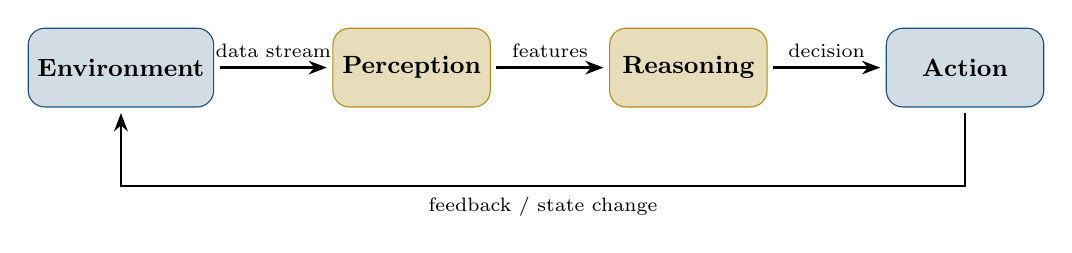
\begin{tikzpicture}[
  node distance=1.5cm,
  box/.style={rectangle, rounded corners=6pt, minimum width=2.0cm, minimum height=1.0cm, align=center, font=\bfseries\small},
  arrow/.style={-Stealth, thick, shorten >=2pt, shorten <=2pt}
]

% Nodes
\node[box, fill=finblue!20, draw=finblue] (env)     {Environment};
\node[box, fill=fingold!30, draw=fingold, right=of env]     (percept) {Perception};
\node[box, fill=fingold!30, draw=fingold, right=of percept] (reason)  {Reasoning};
\node[box, fill=finblue!20, draw=finblue, right=of reason]  (action)  {Action};

% Arrows between nodes
\draw[arrow] (env)     -- node[above, font=\scriptsize] {data stream} (percept);
\draw[arrow] (percept) -- node[above, font=\scriptsize] {features}    (reason);
\draw[arrow] (reason)  -- node[above, font=\scriptsize] {decision}    (action);

% Feedback arrow below
\draw[arrow] (action.south) -- ++(0,-1.0)
             -| node[below, font=\scriptsize, pos=0.25] {feedback / state change} (env.south);

\end{tikzpicture}
\caption{The Perception–Reasoning–Action (PRA) loop, the operational core of every AI agent. In a financial compliance context, the environment is the stream of incoming transactions; the agent continuously monitors, reasons about risk, and acts---filing reports or escalating cases---without awaiting human instruction at each step.}
\label{fig:pra-loop}
\end{figure}

Not all agents are equally autonomous. In practice, financial institutions deploy agents along a spectrum ranging from \textit{assisted} systems, which surface recommendations for human approval, to \textit{fully autonomous} systems, which act without any human checkpoint \cite{shavit2023practices}. Most production deployments today sit in an intermediate zone of \textit{supervised autonomy}: the agent acts independently within tightly defined boundaries, but escalates to a human when it encounters situations outside its confidence threshold or operational mandate.

This spectrum matters for governance. An agent that recommends a trade is subject to a different regulatory regime than one that executes it. Understanding where on the autonomy spectrum a given system sits is therefore not merely a technical question but a legal and ethical one, and this is a theme we return to in Section ~\ref{subsec:governance}.

\section{The Architecture of AI Agents}
\label{sec:architecture}

An agent is not a single, monolithic program. It is an organised collection of specialised modules, each responsible for a distinct stage in the agent's decision-making lifecycle. Understanding this internal structure is essential for anyone who must design, deploy, evaluate, or regulate these systems in a financial context.

Modern agent architectures decompose into five interconnected modules: \textit{perception}, \textit{memory}, \textit{reasoning}, \textit{action}, and \textit{governance}. These modules mirror, at a high level, the cognitive architecture of a skilled human analyst: receiving information from the environment, retaining relevant knowledge, deliberating over options, acting on a decision, and doing so within an institutional framework of rules and oversight. Figure~\ref{fig:agent-architecture} provides a schematic overview of these modules.

The modules do not operate in a simple linear sequence. Reasoning may trigger additional perception (querying a new data source mid-task); memory retrieval informs both what the agent perceives and how it reasons; and governance operates orthogonally to all other modules, monitoring rather than sequencing. This non-linearity is what makes modern agents qualitatively different from classical rule-based systems, which followed rigid if-then pipelines.

\begin{figure}[htbp]
  \centering

% Preamble requirements:
% \usepackage{tikz}
% \usetikzlibrary{positioning,calc}
% \usepackage{xcolor}
% Preamble:
% \usepackage{tikz}
% \usetikzlibrary{positioning,calc}
% \usepackage{xcolor}

% Preamble:
% \usepackage{tikz}
% \usetikzlibrary{positioning}
% \usepackage{xcolor}
% \usepackage{graphicx}

\resizebox{11cm}{!}{
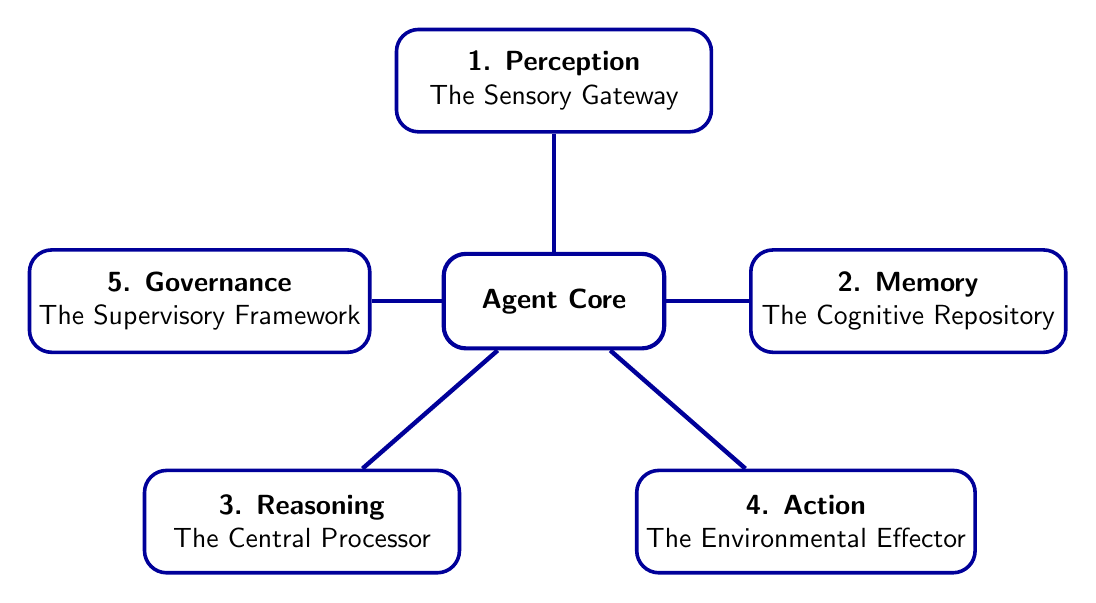
\begin{tikzpicture}[
    font=\sffamily,
    core/.style={
        draw=blue!60!black,
        line width=1.5pt,
        rounded corners=8pt,
        minimum width=2.8cm,
        minimum height=1.2cm,
        align=center
    },
    box/.style={
        draw=blue!60!black,
        line width=1.3pt,
        rounded corners=8pt,
        minimum width=4.0cm,
        minimum height=1.3cm,
        align=center
    },
    conn/.style={
        draw=blue!60!black,
        line width=1.6pt
    }
]

% --- Core
\node[core] (core) at (0,0) {\textbf{Agent Core}};

% --- Top
\node[box] (perception) at (0,2.8) {
\textbf{1. Perception}\\
The Sensory Gateway
};

% --- Left
\node[box] (governance) at (-4.5,0) {
\textbf{5. Governance}\\
The Supervisory Framework
};

% --- Right
\node[box] (memory) at (4.5,0) {
\textbf{2. Memory}\\
The Cognitive Repository
};

% --- Bottom Left
\node[box] (reasoning) at (-3.2,-2.8) {
\textbf{3. Reasoning}\\
The Central Processor
};

% --- Bottom Right
\node[box] (action) at (3.2,-2.8) {
\textbf{4. Action}\\
The Environmental Effector
};

% --- Connections
\draw[conn] (core) -- (perception);
\draw[conn] (core) -- (governance);
\draw[conn] (core) -- (memory);
\draw[conn] (core) -- (reasoning);
\draw[conn] (core) -- (action);

\end{tikzpicture}
}


  \caption{The five-module architecture of a modern AI agent. Information flows from the external world through perception, is stored and retrieved via memory, synthesised into decisions by the reasoning engine, and translated into action. The governance layer wraps the entire lifecycle, enforcing safety and regulatory constraints at every stage.}
  \label{fig:agent-architecture}
\end{figure}

% Not every AI system is an agent. A simple chatbot that responds to a single question and stops is not an agent. A system becomes an \textit{agent} when it satisfies three conditions: (1) it perceives its environment continuously, (2) it selects and executes actions to pursue a goal, and (3) it closes the loop by observing the effects of those actions and adjusting accordingly. This perception-decision-action loop, sustained over time, is the defining characteristic of agency \cite{wooldridge2009introduction}.

% % -----------------------------------------------------------
% \subsection{Perception: The Sensory Gateway}
% \label{subsec:perception}
% % -----------------------------------------------------------

% The \textbf{perception module} is the agent's interface with the external world. It is responsible for ingesting raw, heterogeneous signals from the environment and converting them into structured representations that the reasoning engine can process. Without an effective perception module, even a powerful reasoning engine is blind.

% In financial contexts, the signals an agent must process are remarkably diverse. A trading agent must simultaneously process real-time tick data from exchange feeds, sentiment signals extracted from earnings call transcripts, central bank announcements, and macroeconomic releases. A credit risk agent must ingest structured loan application fields alongside unstructured supporting documentation such as audited financial statements and management letters. A compliance agent must monitor transaction flows and regulatory communications in near-real time.

% Modern perception modules rely on \textbf{transformer-based encoders} to capture the semantic nuance that traditional keyword-based or rule-based parsing would miss \cite{vaswani2017attention}. For example, a rules-based system might treat ``the outlook remains cautious'' and ``the outlook remains stable'' as semantically similar phrases. A transformer-based encoder recognises that these carry meaningfully different implications for monetary policy expectations and, consequently, for asset pricing.

% Beyond raw ingestion, the perception module performs a process called \textbf{semantic grounding}: mapping raw information onto an internal ontology or knowledge graph. When an agent receives the query ``AAPL stock price,'' semantic grounding resolves this to the entity Apple Inc., its exchange identifiers (NASDAQ: AAPL), its sector classification, its relationships to related entities such as its supply chain, and its regulatory filing history. The reasoning engine receives structured, unambiguous information rather than raw text, which substantially improves the reliability of downstream decisions.

% A final and often underappreciated function of the perception module is \textbf{continuous monitoring}, that is the ability to detect material deviations from prior expectations and trigger replanning cycles accordingly. Financial markets are non-stationary environments: correlations shift, liquidity conditions change, and central banks surprise. An agent that perceives the world only at fixed intervals is poorly suited to these dynamics. Continuous monitoring is the financial analogue of a self-driving vehicle detecting an unexpected obstacle and recalculating its route in real time.

% For Example, if we consider a commercial loan underwriting agent at a regional bank. Its perception module must simultaneously ingest: (a) structured data from the loan application form -- revenue, EBITDA, collateral values; (b) unstructured text from the borrower's most recent annual report and management commentary; (c) third-party credit bureau records in XML format; and (d) macroeconomic data feeds indicating current sector conditions. A transformer-based multimodal encoder processes all four streams and produces a unified, structured representation of the borrower's risk profile, which the reasoning engine then evaluates against the bank's credit policy.

% % -----------------------------------------------------------
% \subsection{Memory: The Cognitive Repository}
% \label{subsec:memory}
% % -----------------------------------------------------------

% A single perception-reasoning-action cycle reveals what an agent can do at a given moment. Memory reveals what it can learn and retain over time. Without memory, every interaction starts from scratch. With memory, the agent accumulates experience, recognises patterns across sessions, and becomes progressively more effective at its task.

% Modern agent architectures bifurcate memory into two primary layers that mirror the structure of human cognition \cite{zhao2023survey}.

% \textbf{Short-term (volatile) memory} is implemented through the \textit{context window} of the underlying language model. It retains the immediate dialogue history, in-progress task parameters, and intermediate reasoning steps -- everything the agent requires to maintain coherence within a single session or task. Its fundamental limitation is finite capacity: as context windows fill, older information must be discarded or summarised. For financial agents processing lengthy regulatory documents or extended trading sessions spanning thousands of events, managing this capacity constraint is a genuine and consequential engineering challenge.

% \textbf{Long-term (non-volatile) memory} is implemented through \textit{vector databases} coupled with \textit{Retrieval-Augmented Generation} (RAG) \cite{lewis2020retrieval}. Here the agent stores vast quantities of domain-specific knowledge -- historical market data, regulatory frameworks, counterparty records, past transaction outcomes -- that persist across sessions. When the agent needs relevant information, it converts its current query into a high-dimensional vector and retrieves the most semantically similar content using similarity measures such as cosine similarity or Hierarchical Navigable Small World (HNSW) graphs \cite{malkov2018efficient}. The key insight of RAG is that the agent does not need to memorise everything at training time. Instead, it retrieves relevant knowledge dynamically at inference time, combining the flexibility of a search engine with the reasoning power of a language model.

% % \begin{tcolorbox}[colback=blue!4, colframe=blue!40!black,
% %   title=\textbf{Key Concept: Why RAG Matters for Finance},
% %   fonttitle=\small\bfseries]
% %   \small
% %   Consider the difference between a junior analyst who memorised every regulation from law school (a static, trained model) and one who has access to a constantly updated regulatory database and knows how to search it efficiently (a RAG-enabled agent). The second analyst can handle novel regulatory questions -- even those that did not exist at training time -- by retrieving the relevant guidance before reasoning. For financial agents operating in environments where regulations change frequently, RAG is not an enhancement: it is a necessity.
% % \end{tcolorbox}

% Beyond these two primary layers, specialised memory architectures serve specific purposes. Table~\ref{tab:memory-types} summarises the principal memory types, their implementations, and their financial applications.

% \begin{table}[htbp]
%   \centering
%   \caption{Memory Architectures in Financial AI Agents}
%   \label{tab:memory-types}
%   \renewcommand{\arraystretch}{1.3}
%   \begin{tabular}{|p{2.5cm}|p{3.5cm}|p{5cm}|}
%     \hline
%     \textbf{Type} & \textbf{Implementation} & \textbf{Financial Application} \\
%     \hline
%     Short-term & LLM context window & In-session task coherence, intermediate reasoning steps, active dialogue history \\
%     \hline
%     Long-term & Vector database + RAG & Regulatory frameworks, historical transaction records, counterparty data \\
%     \hline
%     Episodic & Experience replay buffer & Learning from past trades and regulatory inquiries; post-incident review \\
%     \hline
%     Procedural & Policy networks, rule stores & Fast execution of routine compliance checks and standard order types \\
%     \hline
%     Consensus & Shared knowledge base & Multi-agent coordination, preventing contradictory actions across components \\
%     \hline
%   \end{tabular}
% \end{table}

% \textit{Episodic memory} records specific past experiences -- successful and failed trades, regulatory inquiries, client escalations -- enabling the agent to reflect on and learn from its own history, analogous to experience replay in reinforcement learning \cite{mnih2015human}. \textit{Procedural memory} stores learned routines and optimised policies for rapid execution in familiar scenarios, bypassing the computational overhead of full replanning. In multi-agent systems, \textit{consensus memory} provides a shared knowledge base -- a ``single source of truth'' -- that all agents in the ecosystem can read and update, preventing contradictory actions across components \cite{chen2024agentverse}.

% % -----------------------------------------------------------
% \subsection{Reasoning: The Cognitive Core}
% \label{subsec:reasoning}
% % -----------------------------------------------------------

% The \textbf{reasoning engine} is where perception and memory are synthesised into decisions. It is the agent's central processing unit, responsible for evaluating the current state, generating candidate plans, critiquing those plans, and selecting the course of action most likely to achieve the agent's objective.

% \paragraph{Hierarchical Task Decomposition.}

% A foundational reasoning technique is \textit{hierarchical task decomposition}: breaking a complex objective into a directed acyclic graph of manageable sub-tasks. Consider the objective ``produce a comprehensive credit assessment for this corporate borrower.'' This meta-goal decomposes as follows:

% \begin{enumerate}
%   \item Retrieve the borrower's audited financial statements for the past three years.
%   \item Compute liquidity ratios (current ratio, quick ratio), leverage ratios (debt-to-EBITDA), and interest coverage ratios.
%   \item Retrieve industry benchmarks for the borrower's sector and geography.
%   \item Assess qualitative risk factors from management commentary and any available news sources.
%   \item Synthesise quantitative and qualitative findings into a rating recommendation with supporting rationale.
% \end{enumerate}

% Each sub-task may itself decompose further, and the agent tracks dependencies between tasks -- recognising, for example, that the benchmark comparison in step three cannot proceed until ratio analysis in step two is complete. This structured decomposition is what allows agents to tackle objectives far too complex to be addressed in a single reasoning step \cite{huang2024understanding}.

% \paragraph{Metacognition and Self-Critique.}

% Equally important is \textbf{metacognition}: the agent's ability to evaluate its own proposed plans before executing them. A well-designed financial agent does not act on its first plan. It critiques that plan against constraints, risk parameters, and historical failure modes in a ``mental sandbox'' before committing. This self-critique loop is the computational analogue of a portfolio manager who asks ``what could go wrong?'' before entering a position. The Reflexion framework \cite{shinn2023reflexion} formalises this idea, giving agents the ability to generate verbal self-evaluations and iteratively refine their responses. In compliance and document generation tasks, where a single error can carry regulatory consequences, this metacognitive capability is particularly valuable.

% \paragraph{Dynamic Replanning.}

% In non-deterministic environments -- which characterise most financial markets -- the reasoning engine must also perform \textit{dynamic replanning}: continuously reassessing its strategy as new information arrives. Market conditions that prevailed at the start of a trading session may change materially by mid-session. An agent committed to a plan formulated on stale information will underperform or, worse, take actions that are actively harmful. Effective dynamic replanning requires what the planning literature calls ``anytime planning'': the ability to maintain a valid, executable plan at all times, even as the plan is continuously revised \cite{masterman2024landscape}.

% Table~\ref{tab:reasoning-patterns} summarises the principal reasoning patterns available to modern agents, together with their financial applications.

% \begin{table}[htbp]
%   \centering
%   \caption{Reasoning Patterns for Financial AI Agents}
%   \label{tab:reasoning-patterns}
%   \renewcommand{\arraystretch}{1.3}
%   \begin{tabular}{|p{2.8cm}|p{3.7cm}|p{4.5cm}|}
%     \hline
%     \textbf{Pattern} & \textbf{Mechanism} & \textbf{Financial Application} \\
%     \hline
%     ReAct \cite{yao2023react} & Interleaves reasoning traces and actions in a continuous loop & Market surveillance, real-time anomaly detection, live order routing \\
%     \hline
%     Plan-and-Execute & Generates a complete plan prior to any execution step & Regulatory filings, structured report generation, batch processing \\
%     \hline
%     Reflexion \cite{shinn2023reflexion} & Adds explicit self-critique and iterative refinement stages & Compliance analysis, credit memorandum generation \\
%     \hline
%     Tree of Thoughts \cite{yao2023tree} & Explores multiple solution branches simultaneously & Portfolio optimisation, M\&A due diligence, scenario analysis \\
%     \hline
%   \end{tabular}
% \end{table}

% The choice of reasoning pattern is a consequential design decision, not a technical detail. A risk management application where unexpected behaviour carries systemic consequences demands the predictability of Plan-and-Execute. An exploratory research agent seeking novel trading signals may benefit from the breadth of Tree of Thoughts. Mismatching the reasoning pattern to the application context is a common source of agent failure in production deployments.

% \begin{tcolorbox}[colback=yellow!5, colframe=yellow!50!black,
%   title=\textbf{Discussion: Which Reasoning Pattern for Which Task?},
%   fonttitle=\small\bfseries]
%   \small
%   Consider two financial agent tasks: (a) filing a quarterly regulatory report under MiFID II, and (b) scanning the equity market for emerging momentum signals. Which reasoning pattern would you choose for each, and why? Think about what happens if the agent makes an intermediate error in each case, and how each pattern handles error recovery differently.
% \end{tcolorbox}

% % -----------------------------------------------------------
% \subsection{Action: The Effector Module}
% \label{subsec:action}
% % -----------------------------------------------------------

% The \textbf{action module} is where reasoning becomes reality. It translates the agent's digital plans into tangible interventions -- in financial contexts, this might mean executing a trade, issuing a compliance alert, updating a risk model, generating a client report, or querying an external data provider.

% Modern agents achieve this through \textbf{tool use} (also called \textit{function calling}): the ability to invoke external APIs, code interpreters, database queries, and other computational resources \cite{schick2023toolformer}. This capability is what allows an agent to transcend the boundaries of its own trained knowledge and interact with live financial systems. A portfolio management agent that can call a brokerage API to execute orders, query a market data feed for current prices, and write results to a risk management database is qualitatively more capable than one confined to generating text.

% To understand the importance of tool use, consider the analogy of a brilliant financial analyst with no access to a computer, phone, or trading terminal. Their reasoning may be impeccable, but they cannot act in the world. Tool use is the interface between the agent's cognitive capabilities and the external systems that the financial industry runs on.

% \paragraph{Action Taxonomies.}

% The actions available to a financial agent can be organised into four broad categories:

% \begin{itemize}
%   \item \textbf{Data retrieval actions}: querying market data feeds, pulling regulatory filings, fetching counterparty records from internal databases.
%   \item \textbf{Computation actions}: invoking code interpreters to calculate risk metrics, run scenario analyses, or back-test trading strategies.
%   \item \textbf{Transaction actions}: submitting orders to an exchange, initiating payment instructions, updating portfolio records.
%   \item \textbf{Communication actions}: generating client reports, drafting regulatory correspondence, sending alerts to human supervisors.
% \end{itemize}

% \paragraph{Action-Effect Verification.}

% A critical and often overlooked element of the action module is \textbf{action-effect verification}: after taking an action, the agent uses its perception module to confirm that the action achieved its intended outcome. Did the trade execute at the expected price and quantity? Was the report delivered to the correct recipient? Did the database update propagate correctly across all downstream systems? This feedback loop, shown in Figure~\ref{fig:agent-architecture}, enables the agent to initiate corrective cycles when actions fail or produce unexpected outcomes -- a capability that is essential for robustness in complex operational environments \cite{wang2024survey}.

% % -----------------------------------------------------------
% \subsection{Governance: The Supervisory Framework}
% \label{sec:governance}
% % -----------------------------------------------------------

% The \textbf{governance layer} is not a step in the agent's decision cycle: it is a constant supervisor of that cycle. Its purpose is to ensure that all agent operations remain within predefined safety, ethical, and regulatory boundaries. This requirement carries particular weight in financial services, where autonomous decisions can have immediate and material consequences for clients, counterparties, and market stability.

% A common misconception among engineers new to agent design is that governance is something to be added after the agent's capabilities have been fully specified. In practice, the opposite is true: governance constraints should be the first thing specified, because they determine which capabilities are permissible and under what conditions \cite{bai2022constitutional}.

% \paragraph{Constitutional AI.}

% One influential approach to governance is \textbf{Constitutional AI} \cite{bai2022constitutional}, in which proposed actions are evaluated against a set of explicit principles by a secondary ``critic'' model with veto power. In a financial context, these principles might include prohibitions on certain transaction types, position concentration limits, mandatory disclosure requirements, and client communication standards. Any action that violates a principle is blocked before execution, providing a systematic check on the agent's behaviour.

% \paragraph{Regulatory Compliance Enforcement.}

% Agents deployed in financial services must ensure real-time adherence to applicable legal frameworks: MiFID~II transaction reporting requirements, Basel~III capital adequacy rules, GDPR data handling obligations, and AML/KYC screening obligations, among others. Compliance enforcement logic is embedded directly into the governance layer, blocking or flagging actions that would create regulatory exposure before they are executed.

% \paragraph{Human-in-the-Loop Mechanisms.}

% No governance framework for high-stakes financial decisions should rely exclusively on automated controls. \textbf{Human-in-the-Loop (HITL)} mechanisms require mandatory human approval for actions exceeding predefined risk thresholds \cite{wang2024survey}. A credit agent might autonomously approve loans below a certain notional size while escalating larger exposures for human review. A trading agent might execute routine portfolio rebalancing autonomously but require human authorisation for positions above a notional limit or for trades in illiquid instruments. The design of these thresholds -- determining which decisions to automate and which to escalate -- is as much a governance and risk management question as it is a technical one.

% \paragraph{Resource and Budget Management.}

% An often-overlooked governance function is the management of computational resources. An agent consuming unbounded API calls, token budgets, or compute time is itself an operational risk. The governance layer implements throttling, rate limits, and kill switches to prevent runaway processes -- analogous to a circuit breaker in an electrical system.

% \paragraph{Audit Logging and Forensic Traceability.}

% The governance layer maintains tamper-evident, high-fidelity records of every decision trace: the initial trigger, the memory segments retrieved, the full reasoning chain, all tool calls and their outputs, and the final action taken. This forensic traceability is not optional in regulated financial environments. It is the foundation of accountability, the evidence base for regulatory examination, and the starting point for post-incident analysis. In the event that an agent takes an unexpected action, audit logs must be sufficient for supervisors and regulators to reconstruct the decision-making process step by step \cite{novelli2024ai}.

% \begin{tcolorbox}[colback=red!4, colframe=red!40!black,
%   title=\textbf{Key Concept: Governance as a First-Class Design Requirement},
%   fonttitle=\small\bfseries]
%   \small
%   The governance layer wraps the entire agent lifecycle rather than intervening at a single point. An agent without robust governance is not merely a compliance risk: it is an operational liability. In financial services, where regulators expect institutions to be able to explain every material decision, an autonomous system that cannot provide a complete audit trail is, in practice, undeployable -- regardless of its technical performance.
% \end{tcolorbox}

% Table~\ref{tab:governance-mechanisms} summarises the key governance mechanisms and their purposes.

% \begin{table}[htbp]
%   \centering
%   \caption{Governance Mechanisms for Financial AI Agents}
%   \label{tab:governance-mechanisms}
%   \renewcommand{\arraystretch}{1.3}
%   \begin{tabular}{|p{3.2cm}|p{4.3cm}|p{3.5cm}|}
%     \hline
%     \textbf{Mechanism} & \textbf{Purpose} & \textbf{Financial Example} \\
%     \hline
%     Constitutional AI & Enforce explicit ethical and operational rules via a critic model & Block trades that violate concentration limits \\
%     \hline
%     Regulatory compliance & Real-time adherence to legal frameworks & MiFID II transaction reporting, AML screening \\
%     \hline
%     Human-in-the-Loop & Mandatory human approval above risk thresholds & Escalate loans above \$10M to credit committee \\
%     \hline
%     Resource management & Prevent unbounded computational consumption & API call throttling, token budget limits \\
%     \hline
%     Audit logging & Tamper-evident record of every decision step & Full reasoning trace for regulatory examination \\
%     \hline
%   \end{tabular}
% \end{table}

% % -----------------------------------------------------------
% \subsection{Putting the Architecture Together: An End-to-End Example}
% \label{subsec:e2e}
% % -----------------------------------------------------------

% To consolidate understanding of how the five modules interact in practice, consider a simplified end-to-end scenario: a credit underwriting agent evaluating a loan application from a mid-market corporate borrower.

% \begin{enumerate}
%   \item \textbf{Perception}: The agent ingests the loan application form, three years of audited financial statements, and a real-time news feed flagging recent litigation against the borrower. Its transformer-based encoder structures all inputs into a unified risk representation.
%   \item \textbf{Memory}: The agent queries its long-term vector database and retrieves: (a) the regulatory credit policy applicable to this loan category, (b) historical default rates for comparable borrowers in the same sector, and (c) the outcomes of three similar loans approved in the prior year.
%   \item \textbf{Reasoning}: Using a Reflexion-style self-critique loop, the agent decomposes the credit assessment task, computes the relevant financial ratios, compares them against retrieved benchmarks, evaluates the litigation risk, and drafts a preliminary rating recommendation. It then critiques its own recommendation, identifies that the litigation flag warrants additional investigation, and initiates a second retrieval cycle to gather more information.
%   \item \textbf{Action}: The agent generates a structured credit memorandum and, because the loan exceeds the autonomous approval threshold, submits it to a human credit officer for review rather than approving it directly.
%   \item \textbf{Governance}: Throughout all steps, the governance layer verifies that the agent has accessed only data it is authorised to retrieve, that its reasoning complies with the bank's credit policy, and that the full decision trace is captured in the audit log.
% \end{enumerate}

% This example illustrates several important properties of well-designed agent architectures. The modules do not operate in simple linear sequence: the reasoning engine iterates back to memory for additional retrieval, and the governance layer operates continuously across all stages. The agent's decision to escalate to a human reviewer is itself a product of the governance layer's threshold rules, not the reasoning engine's discretion.

% \begin{tcolorbox}[colback=yellow!5, colframe=yellow!50!black,
%   title=\textbf{Practical Activity: Mapping an Agent Architecture to a Financial Use Case},
%   fonttitle=\small\bfseries]
%   \small
%   Select one of the following financial use cases and, for each of the five modules, specify: (a) what inputs or outputs the module would handle, (b) what technologies you would use to implement it, and (c) what could go wrong if that module fails.

%   \begin{itemize}
%     \item A portfolio rebalancing agent for a retail investment platform.
%     \item A real-time AML transaction monitoring agent at a commercial bank.
%     \item A regulatory reporting agent responsible for MiFID II trade reporting.
%   \end{itemize}
% \end{tcolorbox}

% % ============================================================
% % Section: The Architecture of AI Agents
% % Book: AI in Finance
% % ============================================================

% \section{The Architecture of AI Agents}
% \label{sec:architecture}

% Understanding how agents work requires examining their internal structure. Before diving into each component, it is worth stepping back to appreciate the overall design philosophy. A well-engineered AI agent is not a single monolithic program; it is a \textit{system of systems}, a collection of specialized modules that each handle one aspect of intelligent behavior, communicating with one another in a principled way \cite{wooldridge2009introduction}.

% This modular design reflects a lesson learned from decades of AI research and software engineering alike: complex capabilities are best built by composing simpler, well-defined components. Just as a bank separates its front-office trading desk, its back-office settlement team, and its compliance function into distinct organizational units with clear interfaces, a well-architected AI agent separates perception, memory, reasoning, action, and governance into distinct modules with clearly defined inputs and outputs.

% Modern agent architectures decompose into five interconnected modules, each playing a distinct role in the lifecycle of a decision. Figure~\ref{fig:agent-architecture} provides a schematic overview.

% \begin{figure}[htbp]
%   \centering
%   % Replace with actual TikZ diagram or \includegraphics
%   \fbox{\parbox{0.85\textwidth}{\centering\vspace{2cm}
%     [Figure: Agent Architecture --- Perception $\rightarrow$ Memory $\rightarrow$ Reasoning $\rightarrow$ Action,\\
%      wrapped by the Governance layer on all sides]
%   \vspace{2cm}}}
%   \caption{The five-module architecture of a modern AI agent. Arrows represent information flow between modules. The governance layer (Section~\ref{subsec:governance}) wraps the entire decision lifecycle rather than intervening at a single point, auditing and constraining every module continuously.}
%   \label{fig:agent-architecture}
% \end{figure}

% The modules do not operate in a simple linear sequence. Reasoning may trigger additional perception (querying a new data source mid-task); memory retrieval informs both what the agent perceives and how it reasons; and governance operates orthogonally to all other modules, monitoring rather than sequencing. This non-linearity is what makes modern agents qualitatively different from classical rule-based systems, which followed rigid if-then pipelines.

% We examine each module in turn.

% -----------------------------------------------------------
\subsection{Perception: The Sensory Gateway}
\label{subsec:perception}
% -----------------------------------------------------------

The \textbf{perception module} is the agent's interface with the external world. Its job is to take the raw, messy, heterogeneous stream of information that characterizes real financial environments and transform it into clean, structured representations that the reasoning engine can process. Without effective perception, even the most sophisticated reasoning engine is flying blind.

To appreciate why this is non-trivial, consider what a human portfolio manager actually perceives in a single morning: a Bloomberg terminal displaying real-time price feeds; an email from a client expressing concern about her portfolio's energy exposure; a PDF of an earnings release from a major holding; a news alert about a central bank statement; and an internal risk dashboard summarizing overnight position changes. Each of these is a \textit{different modality}, structured numerical data, natural language prose, formatted documents, brief alerts, visual dashboards—and a human integrates them effortlessly. An AI agent must replicate this integration computationally.

Modern perception modules are designed around \textbt{multimodal ingestion}: the ability to process heterogeneous input types simultaneously. In financial contexts, the principal input modalities are:

\begin{itemize}
  \item \textbf{Structured numerical data}: price feeds, order books, financial statement line items, loan application fields, portfolio holdings, and risk metrics. These arrive in tabular or time-series formats and can be ingested directly with minimal preprocessing.
  \item \textbf{Unstructured text}: news articles, analyst reports, earnings call transcripts, regulatory filings, client communications, and legal documents. These require natural language processing before they yield usable signals.
  \item \textbf{Semi-structured data}: JSON and XML feeds from financial data providers, XBRL\footnote{XBRL stands for eXtensible Business Reporting Language} tagged regulatory submissions, and standardized messaging formats such as FIX\footnote{Financial Information eXchange (FIX) protocol } protocol trade confirmations.
  \item \textbf{Document images}: charts, scanned contracts, identity documents, historical records, and handwritten annotations are processed through optical character recognition (OCR) and image analysis.
  \item \textbf{Audio and video}: earnings call audio for tone analysis, recorded advisory conversations for compliance review, and video-based identity verification.
\end{itemize}

Raw ingestion is only the first step. Beyond raw ingestion, the perception module performs \textbt{semantic grounding}: mapping perceived information onto an internal ontology or knowledge graph. For example, the information like ``AAPL stock price'' is grounded to the entity Apple Inc., its exchange identifiers (NASDAQ: AAPL), its sector classification (Technology / Consumer Electronics), and its relationships to related entities (subsidiaries, major suppliers, institutional holders)—supplying the reasoning engine with structured, unambiguous information rather than a raw string.

Raw ingestion constitutes only the initial stage of the pipeline. Beyond simple data acquisition, the perception module performs \textbf{semantic grounding}, that is, the systematic mapping of observed inputs onto an internal ontology or knowledge graph. For instance, the textual input ``AAPL stock price'' is not treated as an isolated string. Instead, it is linked to the canonical entity \emph{Apple Inc.}, enriched with its exchange identifier (NASDAQ: AAPL), sector classification (Technology / Consumer Electronics), and structural relationships to other entities such as subsidiaries, major suppliers, and institutional holders. Through this grounding process, the reasoning engine receives structured, contextually anchored, and unambiguous representations rather than raw textual tokens, thereby enabling more reliable inference and downstream decision-making.

A final core function of the perception module is \textbf{continuous monitoring} and \textbf{change detection}. Financial markets are inherently non-stationary environments in which conditions evolve rapidly and often unexpectedly. Consequently, an agent monitoring a portfolio cannot rely on a single perception step followed by prolonged reasoning. Instead, it must continuously observe its environment, detect deviations from prior expectations, and initiate replanning cycles whenever they occur. From a systems perspective, continuous monitoring is typically realized through \textit{event-driven architectures}. Rather than polling data sources at fixed intervals, such as checking prices every second, the agent subscribes to event streams and is notified only when relevant changes occur. This design simultaneously reduces latency and lowers computational overhead, enabling timely and efficient adaptive behavior.

% \begin{example}[Perception in a Fixed-Income Trading Agent]
% A fixed-income agent monitors sovereign bond markets across twelve countries simultaneously. Its perception module subscribes to real-time yield feeds, processes central bank communication as text, and ingests macroeconomic data releases as structured events. When the U.S. Federal Reserve releases a statement, the perception module: (1) ingests the full text; (2) runs a sentiment and stance classifier to detect hawkish vs. dovish language; (3) grounds mentions of economic indicators to their official statistical definitions; (4) detects that the statement represents a deviation from the prior stance; and (5) triggers a replanning event, passing a structured summary to the reasoning engine within seconds of the release. A human analyst reading the same statement might reach the same qualitative conclusion in five minutes.
% \end{example}

% -----------------------------------------------------------
\subsection{Memory: The Cognitive Repository}
\label{subsec:memory}
% -----------------------------------------------------------
A single perception--reasoning--action cycle reveals what an agent can do \textit{in the moment}. \textbf{Memory} reveals what it can learn and retain \textit{over time}. Without memory, every agent interaction starts from scratch: the agent has no knowledge of past decisions, no record of what worked and what failed, and no understanding of the client it has been serving for five years. This would be the computational equivalent of a portfolio manager who develops amnesia every morning.

Memory is what transforms a reactive system into a \textit{knowledgeable} one. It allows agents to leverage knowledge accumulated over months or years, personalize interactions based on past client history, detect long-run patterns invisible to short-memory systems, and learn from their own mistakes.

\subsubsection{Basic memory types}
Agent architectures typically separate memory into two complementary layers, reflecting well-established distinctions from cognitive psychology \cite{baddeley2025working}.

\begin{itemize}
    \item \textbf{Short-term (volatile) memory.}  Short-term memory is implemented through the \textit{context window} of the underlying language model \cite{brown2020language}. It holds the immediate dialogue history, active task parameters, and intermediate reasoning artifacts, that is, all information required to maintain coherence within a single session or task. Conceptually, it functions as the agent’s ``working desk'': all currently relevant materials are immediately accessible, but the available space is limited. The primary limitation of this memory layer is its finite capacity. As the context window fills, older information must be discarded or condensed. For financial agents that process lengthy regulatory documents, which may span hundreds of pages, or operate during extended trading sessions that generate thousands of price observations, efficient management of this capacity represents a nontrivial engineering challenge. Contemporary state-of-the-art models provide context windows ranging from approximately 128{,}000 to 1{,}000{,}000 tokens. 

    \item \textbf{Long-term (non-volatile) memory.}  Long-term memory is realized through \textit{vector databases} in combination with \textit{Retrieval-Augmented Generation} (RAG) \cite{lewis2020retrieval}. This layer enables the persistent storage of large volumes of domain-specific knowledge, including historical market data, regulatory texts, counterparty information, and prior transaction outcomes. Crucially, this information persists across sessions and remains available after agent restarts. The underlying mechanism merits brief clarification. Information stored in a vector database is first transformed into a high-dimensional numerical representation known as an \textit{embedding vector}, which encodes its semantic content. When the agent later requires relevant knowledge, it converts its current query into an embedding and searches the database for entries with similar meanings. This procedure, referred to as \textit{approximate nearest-neighbor search}, efficiently identifies semantically related information \cite{malkov2018efficient}. The retrieved items are then injected into the agent’s context window, where they can be directly leveraged by the reasoning process.
\end{itemize}

In financial applications, this two-layer memory architecture enables capabilities that would otherwise be infeasible. A credit analysis agent can recall the outcomes of loans issued to comparable borrowers several years earlier. A compliance agent can retrieve the precise regulatory guidance applicable to an unfamiliar transaction structure. A trading agent can access its own historical performance records to identify market conditions under which its strategies have previously underperformed.

\subsubsection{Specialized Memory Types}
Beyond these two primary layers, research in cognitive architectures has identified several specialized memory types that enhance agent performance in particular scenarios \cite{park2023generative}. Table~\ref{tab:memory-types} summarizes these, together with their financial applications.

\begin{table}[htbp]
  \centering
  \caption{Memory Architectures in Financial AI Agents. Each memory type addresses a distinct aspect of an agent’s ability to learn, retain, and apply knowledge over time.}
  \label{tab:memory-types}
  \renewcommand{\arraystretch}{1.4}
  \begin{tabular}{|p{2cm}|p{3.3cm}|p{5.6cm}|}
    \hline
    \textbf{Type} & \textbf{Implementation} & \textbf{Financial Application} \\
    \hline
    Short-term   
      & LLM context window        
      & In-session task coherence and management of intermediate reasoning steps \\
    \hline
    Long-term    
      & Vector database with RAG     
      & Persistent storage of regulatory frameworks, counterparty histories, and market data archives \\
    \hline
    Episodic     
      & Experience replay buffer  
      & Learning from prior trades, post-event adaptation after audits or regulatory inquiries \\
    \hline
    Semantic     
      & Knowledge graph           
      & Representation of entity relationships, market ontologies, and product hierarchies \\
    \hline
    Procedural   
      & Policy networks           
      & Rapid execution of standardized routines such as order routing and report formatting \\
    \hline
    Consensus    
      & Shared knowledge base     
      & Multi-agent coordination and maintenance of consistent market and risk views \\
    \hline
  \end{tabular}
\end{table}

\textit{Episodic memory} records specific past experiences—successful and failed trades, regulatory inquiries, client interactions—and makes them available for reflection and learning. Rather than treating each interaction as isolated, the agent can ask: ``Have I encountered a situation like this before? What happened?''

\textit{Semantic memory} encodes general factual knowledge in a structured knowledge graph: which companies belong to which sector, which regulations apply to which transaction types, which risk factors are correlated. This is distinct from episodic memory (``what happened'') in the same way that a banker's knowledge of how mortgages work is distinct from her memory of a specific mortgage application she processed last month.

\textit{Procedural memory} stores learned routines and optimized policies for rapid execution in familiar scenarios, bypassing the overhead of exhaustive replanning. When a trading agent has executed order routing hundreds of times, it stores the optimized procedure as a callable routine rather than re-deriving it from first principles each time.

In multi-agent systems, \textit{consensus memory} provides a shared knowledge base that all agents in the system can read and write—a ``single source of truth'' that prevents contradictory actions across components. If one agent in a portfolio management system updates its view on interest rate risk, all other agents in the system should be aware of that update before they act.

% -----------------------------------------------------------
\subsection{Reasoning: The Cognitive Core}
\label{subsec:reasoning}
% -----------------------------------------------------------

The \textbf{reasoning engine} is where perception and memory are synthesised
into decisions. If perception is what the agent sees and memory is what the
agent knows, reasoning is what the agent \textit{thinks}. It is the module
responsible for interpreting information, evaluating options, constructing
plans, and deciding on actions.

Reasoning in AI agents draws on a research tradition spanning symbolic AI,
probabilistic inference, and the emergent capabilities of large language
models \cite{wei2022chain}. Modern agents combine these approaches: language
models supply flexible commonsense reasoning, while structured
constraint-satisfaction methods handle problems that require precision and
verifiability.

% ----- 1. Hierarchical Task Decomposition -----

\subsubsection{Hierarchical Task Decomposition}

Complex financial objectives cannot be pursued in a single step. A foundational
reasoning technique is \textit{hierarchical task decomposition}, in which an
agent breaks an open-ended goal into a directed acyclic graph of manageable
sub-tasks \cite{yao2023tree}. This mirrors how skilled professionals approach
complex work: a senior analyst does not attempt to write a credit memorandum
without first gathering data, computing ratios, and benchmarking results.

Consider the goal ``produce a comprehensive credit assessment for a corporate
borrower.'' The agent decomposes this as follows:

\begin{enumerate}
  \item Retrieve the borrower's audited financial statements for the past three
        years.
  \item Compute liquidity ratios (current ratio, quick ratio), leverage ratios
        (debt-to-equity, interest coverage), and profitability metrics
        (EBITDA margin, return on assets).
  \item Retrieve industry benchmark data for each ratio category.
  \item Extract and assess qualitative risk factors from management commentary
        in filings and call transcripts.
  \item Query the long-term memory store for outcomes of comparable prior
        credits.
  \item Synthesise quantitative and qualitative findings into a rating
        recommendation with a confidence interval.
  \item Format the output according to the institution's credit committee
        template.
\end{enumerate}

Each sub-task may further decompose. Step 4, for instance, may branch into
management tenure analysis, strategy assessment, and governance review. The
agent also tracks dependencies among tasks: the benchmark comparison in step 3
cannot meaningfully proceed until the ratio computations in step 2 are
complete.

% ----- 2. Metacognition -----

\subsubsection{Metacognition: Evaluating Plans Before Acting}

A well-designed financial agent does not act on its first plan. Before
committing resources, it runs a self-critique pass in a ``mental sandbox'', evaluating the proposed plan against constraints, risk parameters, and historical failure modes \cite{shinn2023reflexion}. This capacity for \textbf{metacognition} -- reasoning about one's own reasoning -- is what separates a robust agent from a brittle one.

Two complementary mechanisms implement this capability. In \textit{Reflexion}-style architectures \cite{shinn2023reflexion}, the agent generates a plan and then runs a second reasoning pass explicitly tasked with identifying weaknesses, inconsistencies, or constraint violations. 
% In \textit{Constitutional AI} approaches \cite{bai2022constitutional}, the plan is evaluated against a set of explicit principles -- the computational equivalent of asking ``does this plan comply with our investment policy statement?'' -- before any order is submitted. In high-stakes financial contexts, this self-critique loop is not a luxury; it is a necessary safeguard.

% ----- 3. Dynamic Replanning -----

\subsubsection{Dynamic Replanning in Non-Deterministic Environments}

Financial markets are non-deterministic: assumptions embedded in a morning plan may be invalidated by an afternoon announcement. A reasoning engine that commits rigidly to its initial plan is therefore vulnerable to environmental shifts that occur mid-execution.

To address this, agents implement \textit{dynamic replanning} through
\textit{anytime planning} methods \cite{tonola2023anytime}. The agent always maintains a valid current plan and can refine or revise it incrementally as new information arrives, without restarting from scratch. The computational cost of each revision is bounded, ensuring the agent can respond to time-sensitive events without missing their execution window.

% ----- 4. Reasoning Patterns -----

\subsubsection{Reasoning Patterns}

Research has identified several distinct reasoning patterns, each making
different trade-offs between exploration, exploitation, and computational cost.
The appropriate choice is a consequential design decision that should be
aligned with the requirements of the application, not treated as an
implementation detail.

\begin{itemize}
    \item{\textbf{ReAct.}} The ReAct pattern \cite{yao2022react} interleaves reasoning traces and actions in a continuous loop: the agent reasons, takes an action, observes the result, and reasons again. This tight feedback cycle makes it well-suited to applications that require responsiveness to live data, such as market surveillance and real-time anomaly detection, where the agent must continuously update its interpretation as new signals arrive.

    \item{\textbf{Plan-and-Execute.}} The Plan-and-Execute pattern \cite{wang2023plan} separates the work into two distinct phases: the agent first constructs a complete plan, then executes each step in sequence. Because the plan is fully specified before any action is taken, the resulting behaviour is predictable and auditable. This makes it the natural choice for structured, compliance-sensitive workflows such as regulatory filings and periodic reporting, where reproducibility is a requirement.

    \item{\textbf{Reflexion.}} The Reflexion pattern \cite{shinn2023reflexion} introduces an explicit self-critique and iterative refinement loop. After each attempt, the agent evaluates its own output, identifies shortcomings, and produces an improved version. This iterative quality control is particularly valuable in document generation and compliance analysis, where the cost of an error in the final output is high and incremental improvement over multiple passes is feasible.

    \item{\textbf{Tree of Thoughts.}} The Tree of Thoughts pattern \cite{yao2023tree} explores multiple solution branches in parallel, evaluating and pruning weaker paths before committing to a direction. By sampling breadth rather than depth, it is able to discover non-obvious solutions. Applications such as portfolio optimisation and merger and acquisition due diligence -- where the solution space is large and exploratory search is rewarded -- benefit most from this approach.

    \item{\textbf{Chain-of-Thought.}} The Chain-of-Thought pattern \cite{wei2022chain} prompts the model to produce step-by-step intermediate reasoning before arriving at a final answer. Making the reasoning process explicit improves accuracy on multi-step problems and produces an audit trail that analysts and reviewers can inspect. It is the default choice for quantitative analysis and any structured problem-solving task where transparency of reasoning is valued alongside correctness.
\end{itemize}

Mismatching a reasoning pattern to its application is a common source of agent
failure in production systems. A risk management agent, where unexpected
behaviour carries systemic consequences, demands the predictability of
Plan-and-Execute or Chain-of-Thought. An exploratory research agent seeking
novel trading signals may benefit from the breadth of Tree of Thoughts. The
selection should be driven by the operational requirements of the application,
not by the novelty of the method.

\subsubsection{Reasoning Pattern Selection in Practice}

The practical significance of pattern selection becomes clear when examining how a single institution may deploy multiple agents, each requiring a different reasoning approach, for different functions.

Consider a bulge-bracket investment bank that operates two distinct agents in its front and middle offices. Its \textit{compliance monitoring agent} is responsible for reviewing transaction data against a defined set of regulatory rules. Here, predictability and auditability are non-negotiable: every decision must be fully traceable and explainable to regulators upon request. The Plan-and-Execute pattern is the appropriate choice. The agent generates a complete, structured reasoning plan before examining any transaction record, producing a documented chain of logic that can be reviewed step by step long after the decision was made.

Its \textit{equity research agent} faces an entirely different challenge. When a company publishes its quarterly earnings release, the relevant question is not whether a rule has been violated, but what the results mean across a range of possible interpretations. The agent must simultaneously develop a bull case grounded in stronger-than-expected revenue growth, a bear case centred on margin compression and rising costs, and a base case that weighs these signals against consensus expectations. The Tree of Thoughts pattern serves this goal well: the agent explores each interpretive branch in parallel, evaluates the evidence supporting each, and synthesises the findings into a balanced research note. The exploratory, multi-branch structure of this pattern would be poorly suited to the compliance task, just as the rigid sequential structure of Plan-and-Execute would be poorly suited to this one.

This contrast illustrates a general principle: the reasoning pattern is not a technical implementation choice made once at deployment. It is an architectural decision that must be revisited for each agent and each task type, guided by the operational requirements of the application. Getting this decision right is one of the most consequential responsibilities of the agent designer.


% -----------------------------------------------------------
\subsection{Action: The Effector Module}
\label{subsec:action}
% -----------------------------------------------------------
The \textbf{action module} is where reasoning becomes reality. It translates the agent's digital plans into tangible interventions in the world—in financial contexts, this might mean executing a trade, issuing a compliance alert, updating a risk model, generating a client report, querying an external data source, or sending a communication. Action is the module that makes an agent consequential.

This consequentiality is precisely what distinguishes an agent from a conventional AI model and what makes governance so important. A language model that generates an erroneous analysis causes no direct harm until a human acts on it; an agent that executes a trade based on an erroneous analysis causes immediate, material harm without any intervening human decision.

\subsubsection{Tool Use and Function Calling}

Modern agents achieve their action capability through \textit{tool use} (also called \textit{function calling}): the ability to invoke external APIs, code interpreters, database queries, and other computational resources \cite{schick2023toolformer}. This is what allows an agent to transcend the boundaries of its own trained knowledge and interact with live financial systems.

A portfolio agent that can call a brokerage API to execute orders, query a market data feed for current prices, run a Python code interpreter to perform custom quantitative analysis, and write results to a risk management database is qualitatively more capable than one confined to generating text. The tool ecosystem effectively extends the agent's capabilities indefinitely, limited only by the interfaces available.

Common tool categories in financial agent deployments include:

\begin{itemize}
  \item \textbf{Market data APIs}: real-time and historical price feeds, order book data, alternative data sources.
  \item \textbf{Execution interfaces}: brokerage APIs, Financial Information Exchange (FIX) protocol connections, OMS (order management system) integrations.
  \item \textbf{Analytical tools}: code interpreters for statistical computation, optimization solvers, risk models.
  \item \textbf{Document tools}: PDF parsers, OCR engines, template renderers for report generation.
  \item \textbf{Communication interfaces}: email, secure messaging, CRM system updates, regulatory reporting portals.
  \item \textbf{Internal databases}: position management systems, client records, compliance databases.
\end{itemize}

\subsubsection{Action--Effect Verification}

A critical element of the action module is \textbf{action--effect verification}: after taking an action, the agent uses its perception module to confirm that the action achieved its intended outcome. Did the trade execute at the expected price, or did it experience slippage? Was the report delivered successfully? Did the database update propagate correctly? Was the regulatory filing acknowledged by the recipient system?

This feedback loop enables corrective cycles when actions fail or produce unintended results, providing robustness in complex operational environments where partial failures are common. Without verification, an agent can enter an inconsistent state, believing it has completed a task when it has not. A compliance agent that believes it has filed a required report but has not is an operational and regulatory liability.

\subsubsection{Action Hierarchies and Reversibility}

Not all actions carry equal risk. A well-designed action module respects an \textit{action hierarchy} that classifies actions by their reversibility and the magnitude of their consequences. At the top of the hierarchy sit irreversible, high-consequence actions (executing a large trade, filing a regulatory document, disbursing a loan); at the bottom sit reversible, low-consequence actions (retrieving data, generating a draft, running an analysis). Governance thresholds, discussed in the following section, are typically calibrated to this hierarchy, requiring progressively greater authorization as the magnitude of the consequences and the irreversibility of the proposed action increase.

% -----------------------------------------------------------
\subsection{Governance: The Supervisory Framework}
\label{subsec:governance}
% -----------------------------------------------------------
The \textbf{governance layer} is not a step in the agent's decision cycle but rather a \textit{constant supervisor} of that cycle. Its purpose is to ensure that all agent operations remain within predefined safety, ethical, and regulatory boundaries—a requirement that carries particular weight in financial services, where autonomous decisions can have immediate, material, and systemic consequences.

A useful framing is that the governance is to an AI agent what a risk management framework is to a trading desk. A trading desk without position limits, stop-loss rules, and compliance oversight is not merely an operational risk, it is an accident waiting to happen. The 2010 Flash Crash, in which algorithmic trading systems interacted in unanticipated ways to briefly erase nearly \$1 trillion in market value \cite{kirilenko2017flash}, illustrates what inadequately governed automated systems can produce at scale.

Governance should be designed \textit{before} an agent's capabilities are fully specified, not retrofitted afterward. Retrofitting governance onto a capable agent is like installing brakes on a moving car, technically possible, but far more dangerous and far less reliable than building them into the design from the start.

\subsubsection{Constitutional AI and Principle-Based Constraints}
\label{governance}
\textbf{Constitutional AI} \cite{bai2022constitutional} is a governance approach in which proposed actions are evaluated against an explicit set of rules or principles—a ``constitution'', before execution, often using a secondary ``critic'' model with veto power over the primary agent.

In a financial context, the agent's constitution might include principles such as:
\begin{itemize}
  \item ``Do not recommend or execute any transaction that would result in a net portfolio concentration exceeding 10\% in any single issuer.''
  \item ``Flag any communication with a client that contains forward-looking performance claims for human review before sending.''
  \item ``Do not process any transaction involving a counterparty on the OFAC Specially Designated Nationals list.''
  \item ``Escalate any credit decision involving a loan above \$5 million to a senior credit officer regardless of assessed risk.''
\end{itemize}

Each proposed action passes through a constitutional evaluation step. Actions that violate a principle are blocked or flagged; actions that are ambiguous with respect to a principle are escalated for human review; clearly compliant actions proceed. This approach provides a principled, auditable mechanism for encoding institutional policies into agent behavior.

\subsubsection{Regulatory Compliance Enforcement}

Financial services is one of the most heavily regulated industries in the world. AI agents operating in this environment must navigate a complex, overlapping web of regulatory requirements—and compliance cannot be an afterthought.

The governance layer enforces real-time adherence to applicable legal frameworks, including:

\begin{itemize}
  \item \textbf{MiFID II} (Markets in Financial Instruments Directive): best execution obligations, transaction reporting, product governance.
  \item \textbf{Basel III/IV}: capital adequacy requirements, leverage ratios, liquidity coverage.
  \item \textbf{GDPR} (General Data Protection Regulation): data minimization, purpose limitation, right to explanation for automated decisions.
  \item \textbf{AML/KYC} (Anti-Money Laundering / Know Your Customer): transaction monitoring, suspicious activity reporting, customer due diligence.
  \item \textbf{Dodd-Frank / EMIR}: derivatives reporting, central clearing obligations, position limits.
\end{itemize}

Crucially, the ``right to explanation'' embedded in GDPR and emerging AI regulations \cite{act2024eu} places a specific technical requirement on financial AI agents: they must be capable of generating human-intelligible explanations for consequential automated decisions. This is not merely a governance preference; it is a legal obligation in many jurisdictions.

\subsubsection{Human-in-the-Loop Mechanisms}

Governance does not require that every agent action be approved by a human—that would negate the efficiency rationale for deploying agents in the first place. Instead, effective governance implements \textit{tiered} Human-in-the-Loop (HITL) mechanisms calibrated to risk level \cite{cihon2021corporate}.

A typical tiered HITL design for a credit underwriting agent might operate as follows:
\begin{itemize}
  \item \textbf{Tier 1} (fully autonomous): Loans below \$100,000 with risk score above threshold; agent approves, notifies, and documents.
  \item \textbf{Tier 2} (supervised autonomy): Loans between \$100,000 and \$1 million—agent generates recommendation with full reasoning trace; officer approves or overrides within a defined SLA.
  \item \textbf{Tier 3} (human-led, agent-assisted): Loans above \$1 million or with unusual risk factors; the credit committee decides, the agent provides analysis and answers queries.
\end{itemize}

This design ensures that human judgment is concentrated where it adds the most value—in complex, high-stakes decisions—while freeing human capacity from routine decisions where the agent's judgment is both faster and more consistent.

\subsubsection{Resource Management and Kill Switches}

The governance layer also manages \textbf{resource consumption}. An agent that consumes unbounded computational resources by making thousands of unnecessary API calls, running indefinitely without making progress, or accumulating massive context windows, is an operational risk. Production governance systems need to implement:

\begin{itemize}
    \item  \textbf{Resource and budget management.} The agent tracks computational costs (token usage, API calls) and implements throttling to limit total token usage per task.
  \item \textbf{Timeout mechanisms}: maximum execution time per task, after which the agent is interrupted, and the partial result is escalated.
  \item \textbf{Kill switches}: immediate halt mechanisms triggerable by human operators or by automated anomaly detection systems.
\end{itemize}

Kill switches, in particular, are a non-negotiable safety feature for any autonomous agent operating in a live financial environment. The ability to immediately halt an agent that is behaving unexpectedly, without waiting for it to complete its current task, is the last line of defense against compounding errors.

\subsubsection{Audit Logging and Forensic Traceability}

The governance layer maintains \textbf{tamper-evident, high-fidelity audit logs} of every decision trace: the initial trigger and its raw inputs, the memory segments retrieved during reasoning, the full reasoning chain and any intermediate critiques, all tool calls made and their outputs, governance checks applied and their results, and the final action taken along with its verification outcome.

This forensic traceability is not optional in regulated financial environments; it is the foundation of accountability. When a regulator asks ``why did your agent flag this transaction?'' or ``why did your system recommend this trade?'', the audit log must be able to answer that question completely and verifiably. When an unexpected loss occurs, the audit log is the starting point for post-incident analysis. When a client disputes an automated decision, the audit log is the evidence that the decision was made correctly and in accordance with applicable rules.

Technically, audit logs for financial AI agents must satisfy several requirements beyond those of conventional system logs, they must be:
\begin{itemize}
    \item \textbf{immutable}: tamper-evident through cryptographic hashing 
    \item \textbf{complete}: capturing the full reasoning chain, not just inputs and outputs, 
    \item \textbf{human-intelligible}: admissible as regulatory evidence 
    \item \textbf{retained}: for the duration required by applicable regulations (typically three to seven years for most financial records).
\end{itemize}


% \begin{table}[htbp]
%   \centering
%   \caption{Governance Mechanisms for Financial AI Agents. Collectively, these mechanisms provide the institutional safeguards required to make autonomous financial agents operationally viable.}
%   \label{tab:governance}
%   \renewcommand{\arraystretch}{1.4}
%   \begin{tabular}{|p{3.5cm}|p{8cm}|}
%     \hline
%     \textbf{Mechanism} & \textbf{Purpose and Implementation} \\
%     \hline
%     Constitutional AI      
%       & Principle-based pre-action evaluation enforced through a critic model with explicit veto authority \\
%     \hline
%     Regulatory enforcement 
%       & Continuous, real-time compliance verification against regulatory frameworks such as MiFID II, Basel III, GDPR, and AML/KYC \\
%     \hline
%     Tiered HITL            
%       & Risk-calibrated human-in-the-loop approval thresholds with mandatory escalation when predefined limits are exceeded \\
%     \hline
%     Resource management    
%       & Explicit control of computational and operational resources, including token budgets, API rate limits, execution timeouts, and operator-activated kill switches \\
%     \hline
%     Audit logging          
%       & Tamper-evident, complete, and human-interpretable decision traces enabling full post hoc auditability and forensic accountability \\
%     \hline
%     Anomaly detection      
%       & Automated monitoring to identify behavioral drift, policy violations, or out-of-distribution agent actions in real time \\
%     \hline
%   \end{tabular}
% \end{table}

\subsubsection{Designing for Governance from the Start}

A recurring mistake in financial AI deployments is treating governance as a feature to be added after the agent is built. This approach consistently produces fragile, inadequate safeguards. Effective governance requires that the agent's internal representations be \textit{interpretable}, its decision boundaries be \textit{explicit}, and its reasoning be \textit{logged at the right level of granularity} from the outset. These are design choices, not post-hoc additions. Building a financial AI agent without governance in mind from day one is not a development shortcut, it is a liability. The governance layer wraps the entire agent lifecycle rather than intervening at a single point. An agent without robust governance is not merely a compliance risk; it is an operational liability and, in systemic terms, a potential threat to market stability. 



% % --------------------------------------------
% \section{The Architecture of AI Agents}
% \label{sec:architecture}

% Understanding how agents work requires examining their internal structure. Modern agent architectures decompose into five interconnected modules, each playing a distinct role in the lifecycle of a decision. Figure~\ref{fig:agent-architecture} provides a schematic overview.

% \begin{figure}[htbp]
%   \centering
%   % Replace with actual TikZ diagram or \includegraphics
%   \fbox{\parbox{0.85\textwidth}{\centering\vspace{2cm}
%     [Figure: Agent Architecture — Perception $\rightarrow$ Memory $\rightarrow$ Reasoning $\rightarrow$ Action, wrapped by Governance]
%   \vspace{2cm}}}
%   \caption{The five-module architecture of a modern AI agent. The governance layer (Section~\ref{sec:governance}) wraps the entire decision lifecycle rather than intervening at a single point.}
%   \label{fig:agent-architecture}
% \end{figure}

% \subsection{Perception: The Sensory Gateway}


% The \textbf{perception module} is the agent's interface with the external world. It ingests heterogeneous, multimodal signals—structured data such as price feeds and financial statements; unstructured data such as news articles, analyst reports, and regulatory filings; and, in some applications, audio or visual inputs—and converts them into structured representations that the reasoning engine can process.

% In financial contexts, the sophistication of the perception module is critical. A trading agent must process real-time tick data alongside sentiment signals extracted from earnings call transcripts. A credit risk agent must ingest both structured loan application fields and unstructured supporting documentation. Modern perception modules employ transformer-based encoders to capture semantic nuance that traditional keyword-based parsing would miss—understanding, for example, that ``the outlook remains cautious'' in a central bank statement carries meaningfully different implications from ``the outlook remains stable.''

% Beyond raw ingestion, the perception module performs \textit{semantic grounding}: mapping perceived information onto an internal ontology or knowledge graph. A query for ``AAPL stock price'' is grounded to the entity Apple Inc., its exchange identifiers, its sector classification, and its relationships to related entities—supplying the reasoning engine with structured, unambiguous information rather than raw text.

% Equally important is \textbf{continuous monitoring}. Financial markets are non-stationary environments: conditions change, and agents must detect material deviations from prior expectations and trigger replanning cycles accordingly. This is the financial analogue of a self-driving system detecting an unexpected obstacle and recalculating its route.


% \subsection{Memory: The Cognitive Repository}
% \label{subsec:memory}


% A single perception–reasoning–action cycle reveals what an agent can do in the moment. Memory reveals what it can learn and retain over time. Modern agent architectures bifurcate memory into two layers that mirror human cognitive architecture.

% \textbf{Short-term (volatile) memory} is implemented through the \textit{context window} of the underlying language model. It retains the immediate dialogue history, in-progress task parameters, and intermediate reasoning steps—everything the agent requires to maintain coherence within a single session or task. Its limitation is finite capacity: as context windows fill, older information must be discarded or summarized. For financial agents processing lengthy regulatory documents or extended trading sessions, managing this capacity efficiently is a genuine engineering challenge.

% \textbf{Long-term (non-volatile) memory} is implemented through \textit{vector databases} coupled with \textit{Retrieval-Augmented Generation} (RAG). Here the agent stores vast quantities of domain-specific knowledge—historical market data, regulatory frameworks, counterparty records, past transaction outcomes—that persist across sessions. When the agent requires relevant information, it vectorizes its current query and retrieves the most semantically similar content using indexing methods such as cosine similarity or Hierarchical Navigable Small World (HNSW) graphs \citep{malkov2018efficient}.

% For financial agents, this architecture enables capabilities that would otherwise be impossible. A credit analyst agent can recall the outcomes of loans made to comparable borrowers three years prior. A compliance agent can retrieve the specific regulatory guidance applicable to a novel transaction type. A trading agent can access its own historical performance data to refine its decision-making heuristics.

% Beyond these two primary layers, specialized memory architectures serve specific purposes, as summarized in Table~\ref{tab:memory-types}.

% \begin{table}[htbp]
%   \centering
%   \caption{Memory Architectures in Financial AI Agents}
%   \label{tab:memory-types}
%   \renewcommand{\arraystretch}{1.3}
%   \begin{tabular}{llp{6cm}}
%     \toprule
%     \textbf{Type} & \textbf{Implementation} & \textbf{Financial Application} \\
%     \midrule
%     Short-term   & LLM context window       & In-session task coherence, intermediate reasoning \\
%     Long-term    & Vector database + RAG    & Regulatory frameworks, historical transaction data \\
%     Episodic     & Experience replay buffer & Learning from past trades, regulatory inquiries \\
%     Procedural   & Policy networks          & Fast execution of familiar routines \\
%     Consensus    & Shared knowledge base    & Multi-agent coordination and consistency \\
%     \bottomrule
%   \end{tabular}
% \end{table}

% \textit{Episodic memory} records specific past experiences—successful and failed trades, regulatory inquiries, client interactions—enabling reflection and learning analogous to experience replay in reinforcement learning. \textit{Procedural memory} stores learned routines and optimized policies for rapid execution in familiar scenarios, bypassing the overhead of exhaustive replanning. In multi-agent systems, \textit{consensus memory} provides a shared knowledge base—a ``single source of truth''—that all agents in the system can read and update, preventing contradictory actions across components.


% \subsection{Reasoning: The Cognitive Core}
% \label{subsec:reasoning}


% The \textbf{reasoning engine} is where perception and memory are synthesized into decisions. It is the agent's central processing unit, employing deductive, inductive, or abductive logic to formulate plans and evaluate candidate actions.

% A foundational technique is \textit{hierarchical task decomposition}: breaking complex objectives into directed acyclic graphs of manageable sub-tasks. Consider the objective ``produce a comprehensive credit assessment for this corporate borrower.'' This meta-goal decomposes as follows:

% \begin{enumerate}
%   \item Retrieve the borrower's financial statements.
%   \item Compute liquidity, leverage, and interest coverage ratios.
%   \item Retrieve industry benchmarks for comparison.
%   \item Assess qualitative risk factors from management commentary.
%   \item Synthesize findings into a rating recommendation.
% \end{enumerate}

% Each sub-task may itself decompose further, and the agent tracks dependencies between tasks—recognizing, for example, that the benchmark comparison cannot proceed until ratio analysis is complete.

% Equally important is \textbf{metacognition}: the ability to evaluate proposed plans before executing them. A well-designed financial agent does not act on its first plan—it critiques that plan against constraints, risk parameters, and historical failure modes in a ``mental sandbox'' before committing. This self-critique loop is the computational analogue of a portfolio manager asking ``what could go wrong?'' before entering a position.

% In non-deterministic environments—which characterize most financial markets—the reasoning engine must also perform \textit{dynamic replanning}: continuously reassessing its strategy as new information arrives, using ``anytime planning'' methods that always maintain a valid path forward even as conditions evolve.

% Table~\ref{tab:reasoning-patterns} summarizes the principal reasoning patterns available to modern agents, together with their appropriate financial applications.

% \begin{table}[htbp]
%   \centering
%   \caption{Reasoning Patterns for Financial AI Agents}
%   \label{tab:reasoning-patterns}
%   \renewcommand{\arraystretch}{1.3}
%   \begin{tabular}{lp{4.5cm}p{5cm}}
%     \toprule
%     \textbf{Pattern} & \textbf{Mechanism} & \textbf{Suitable Financial Application} \\
%     \midrule
%     ReAct             & Interleaves reasoning and action in a continuous loop          & Market surveillance, anomaly detection \\
%     Plan-and-Execute  & Generates a complete plan prior to execution                   & Regulatory filings, structured workflows \\
%     Reflexion         & Adds an explicit self-critique and refinement stage            & Document generation, compliance analysis \\
%     Tree of Thoughts  & Explores multiple solution paths simultaneously                & Portfolio optimization, M\&A due diligence \\
%     \bottomrule
%   \end{tabular}
% \end{table}

% The choice of reasoning pattern is a consequential design decision, not a technical detail. A risk management application where unexpected behavior carries systemic consequences demands the predictability of Plan-and-Execute. An exploratory research agent seeking novel trading signals may benefit from the breadth of Tree of Thoughts. Mismatching pattern to application is a common source of agent failure in production systems.

% \subsection{Action: The Effector Module}
% \label{subsec:action}

% The \textbf{action module} is where reasoning becomes reality. It translates digital plans into tangible interventions—in financial contexts, this might mean executing a trade, issuing a compliance alert, updating a risk model, generating a client report, or querying an external data source.

% Modern agents achieve this through \textit{tool use} (also called \textit{function calling}): the ability to invoke external APIs, code interpreters, database queries, and other computational resources. This is what allows an agent to transcend the boundaries of its own trained knowledge and interact with live financial systems. A portfolio agent that can call a brokerage API to execute orders, query a market data feed for current prices, and write results to a risk management database is qualitatively more capable than one confined to generating text.

% A critical element of the action module is \textbf{action–effect verification}: after taking an action, the agent uses its perception module to confirm that the action achieved its intended outcome. Did the trade execute at the expected price? Was the report delivered successfully? Did the database update propagate correctly? This feedback loop enables corrective cycles when actions fail, providing robustness in complex operational environments.


% \subsection{Governance: The Supervisory Framework}
% \label{sec:governance}


% The \textbf{governance layer} is not a step in the agent's decision cycle but a constant supervisor of it. Its purpose is to ensure that all agent operations remain within predefined safety, ethical, and regulatory boundaries—a requirement that carries particular weight in financial services, where autonomous decisions can have immediate and material systemic consequences.

% Key governance mechanisms include the following.

% \textbf{Constitutional AI.} Proposed actions are evaluated against explicit rules or principles, often using a secondary ``critic'' model with veto power. In a financial context, these rules might include prohibitions on certain transaction types, position concentration limits, or client communication standards \citep{bai2022constitutional}.

% \textbf{Regulatory compliance enforcement.} The agent ensures real-time adherence to applicable legal frameworks—MiFID~II, Basel~III, GDPR, AML/KYC requirements—blocking or flagging actions that would create regulatory exposure before they are executed.

% \textbf{Human-in-the-Loop (HITL) mechanisms.} Mandatory human approval is required for actions exceeding predefined risk thresholds. A credit agent might autonomously approve loans below a certain size while escalating larger exposures for human review; a trading agent might execute routine rebalancing autonomously but require human authorization for positions above a notional limit.

% \textbf{Resource and budget management.} The agent tracks computational costs (token usage, API calls) and implements throttling or kill switches to prevent runaway processes. In production financial systems, an agent consuming unbounded computational resources is itself an operational risk.

% \textbf{Audit logging.} The system maintains tamper-evident, high-fidelity records of every decision trace: the initial trigger, the memory segments retrieved, the full reasoning chain, all tool calls and their outputs, and the final action taken. This forensic traceability is not optional in regulated financial environments—it is the foundation of accountability, the evidence base for regulatory examination, and the starting point for post-incident analysis.

% The governance layer wraps the entire agent lifecycle rather than intervening at a single point. An agent without robust governance is not merely a compliance risk—it is an operational liability. In practice, governance should be designed before the agent's capabilities are fully specified, not retrofitted afterward.

% -----------------------

% ================================================================
\section{Connecting Agents to the World: Protocols for Integration and Collaboration}
\label{sec:agent-protocols}

The previous sections described how an AI agent reasons, remembers, and acts. Two practical questions follow naturally. First: how does an agent connect to the external systems it must interact with, such as market data feeds, credit databases, regulatory portals, and trade execution platforms? Second: how do multiple agents coordinate when a task exceeds the capacity of any single agent?

This section addresses both questions through two complementary open standards. The \textbf{Model Context Protocol (MCP)\footnote{https://modelcontextprotocol.io/}} solves the first problem by standardizing how an agent integrates with external tools and data sources \cite{hou2025model}. The \textbf{Agent2Agent Protocol (A2A)}\footnote{https://a2a-protocol.org} solves the second by standardizing how agents communicate with each other. Together, they form the communication backbone of modern, enterprise-grade AI deployments in financial services. 

\subsection{The Integration Problem}
\label{sec:mcp-integration-problem}

Before MCP, connecting an AI agent to external data sources and tools required a custom connector for every pair of systems to be integrated. A bank deploying an AI agent might need it to connect to a Bloomberg terminal, an internal credit database, a regulatory reporting portal, a core banking system, and a document management platform. Each connection demanded its own authentication method, data format, and error-handling logic.

This pattern is known as the \textbf{N$\times$M integration problem}: if there are $N$ AI applications and $M$ external tools or data sources, building direct custom connectors between every pair requires up to $N \times M$ distinct integrations. For a medium-sized financial institution with dozens of AI applications and hundreds of internal and external data systems, this multiplication quickly becomes unmanageable.

Figure~\ref{fig:mcp-nm-problem} illustrates how MCP collapses this complexity. Rather than $N \times M$ custom connectors, each AI application implements the MCP client standard once, and each external tool or data source implements the MCP server standard once. Any compliant client can then communicate with any compliant server, reducing the total integration burden from $N \times M$ to $N + M$.

\begin{figure}[h!]
\centering
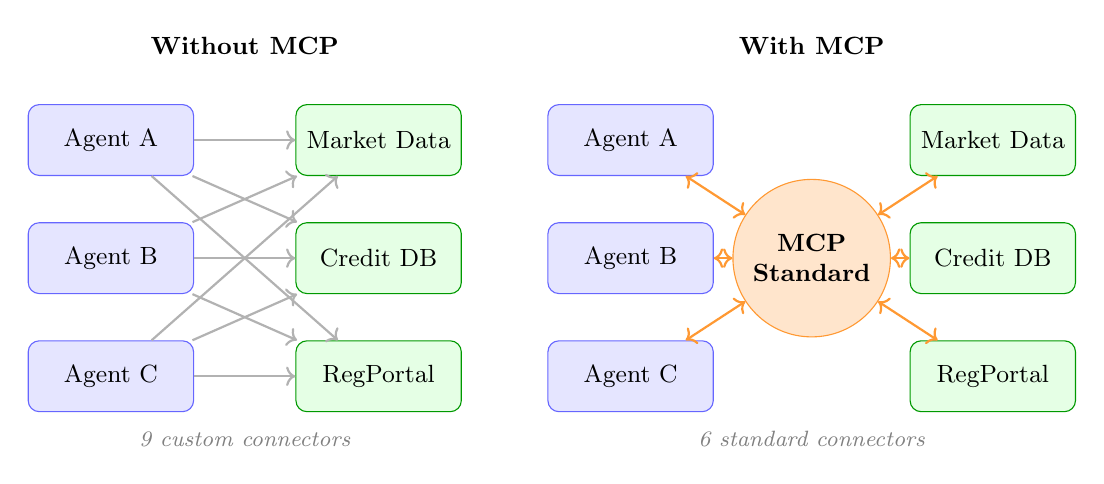
\begin{tikzpicture}[
app/.style={
  rectangle,
  rounded corners,
  draw=blue!60,
  fill=blue!10,
  minimum width=2.1cm,
  minimum height=0.9cm,
  inner sep=2pt,
  font=\small
},
tool/.style={
  rectangle,
  rounded corners,
  draw=green!60!black,
  fill=green!10,
  minimum width=2.1cm,
  minimum height=0.9cm,
  inner sep=2pt,
  font=\small
},
  hub/.style={
    circle,
    draw=orange!80,
    fill=orange!20,
    minimum size=2.0cm,
    font=\small\bfseries,
    align=center
  },
  arr/.style={->, thick, gray!60},
  mcparr/.style={<->, thick, orange!80}
]

% ---- LEFT SIDE: Without MCP (N x M tangle) ----
\node[font=\bfseries\small] at (-4.5, 3.5) {Without MCP};

\node[app] (a1) at (-6.2,  2.3) {Agent A};
\node[app] (a2) at (-6.2,  0.8) {Agent B};
\node[app] (a3) at (-6.2, -0.7) {Agent C};

\node[tool] (t1) at (-2.8,  2.3) {Market Data};
\node[tool] (t2) at (-2.8,  0.8) {Credit DB};
\node[tool] (t3) at (-2.8, -0.7) {RegPortal};

\draw[arr] (a1) -- (t1);
\draw[arr] (a1) -- (t2);
\draw[arr] (a1) -- (t3);
\draw[arr] (a2) -- (t1);
\draw[arr] (a2) -- (t2);
\draw[arr] (a2) -- (t3);
\draw[arr] (a3) -- (t1);
\draw[arr] (a3) -- (t2);
\draw[arr] (a3) -- (t3);

\node[font=\footnotesize\itshape, gray] at (-4.5, -1.5) {9 custom connectors};

% ---- RIGHT SIDE: With MCP (hub) ----
\node[font=\bfseries\small] at (2.7, 3.5) {With MCP};

\node[app] (b1) at (0.4,  2.3) {Agent A};
\node[app] (b2) at (0.4,  0.8) {Agent B};
\node[app] (b3) at (0.4, -0.7) {Agent C};

\node[hub] (mcp) at (2.7, 0.8) {MCP\\Standard};

\node[tool] (s1) at (5.0,  2.3) {Market Data};
\node[tool] (s2) at (5.0,  0.8) {Credit DB};
\node[tool] (s3) at (5.0, -0.7) {RegPortal};

\draw[mcparr] (b1) -- (mcp);
\draw[mcparr] (b2) -- (mcp);
\draw[mcparr] (b3) -- (mcp);
\draw[mcparr] (mcp) -- (s1);
\draw[mcparr] (mcp) -- (s2);
\draw[mcparr] (mcp) -- (s3);

\node[font=\footnotesize\itshape, gray] at (2.7, -1.5) {6 standard connectors};

\end{tikzpicture}
\caption{The N$\times$M integration problem and how MCP resolves it. Without a standard protocol, three agents connecting to three tools require nine custom connectors. With MCP, each side implements the standard once, reducing the total to six standard connections, a saving that grows dramatically as the number of agents and tools increases.}
\label{fig:mcp-nm-problem}
\end{figure}

% ----------------------------------------------------------------
\subsection{The Model Context Protocol}
\label{sec:mcp}

The \textbf{Model Context Protocol (MCP)} is an open standard that defines how AI systems integrate with external data sources, tools, and services \cite{anthropicmcp2024}. Introduced by Anthropic in November 2024, it was subsequently adopted by major AI providers including OpenAI and Google DeepMind. In December 2025, governance transferred to the Agentic AI Foundation under the Linux Foundation, establishing it as a vendor-neutral community standard.

A useful analogy is the \textbf{USB-C standard} for hardware peripherals. Before USB-C, connecting a device to a computer required different cables and ports depending on the manufacturer. USB-C replaced this fragmentation with a single universal connector: any device that implements the standard can plug into any compliant port. MCP serves the same role for AI agents: any agent that speaks MCP can connect to any tool or data source that also speaks MCP, regardless of the underlying technology. Technically, MCP is built on JSON-RPC 2.0, a lightweight remote procedure call protocol that uses JSON as its data format \cite{mcpspec2025}.

\subsubsection{The MCP Architecture}

MCP defines a three-component architecture, illustrated in Figure~\ref{fig:mcp-architecture}.



\begin{figure}[h!]
\centering
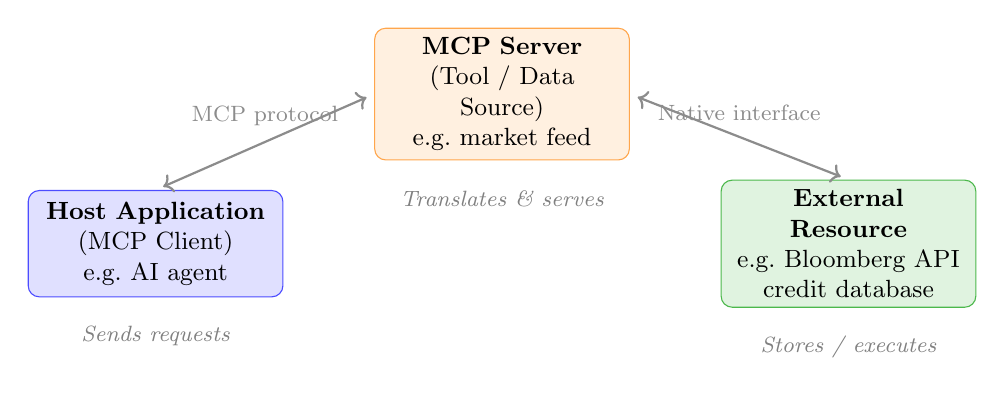
\begin{tikzpicture}[
  box/.style={
    rectangle,
    rounded corners=4pt,
    draw=#1!70,
    fill=#1!12,
    minimum width=3.2cm,
    minimum height=1.35cm,
    text width=3.0cm,
    align=center,
    font=\small
  },
  lbl/.style={font=\footnotesize\itshape, gray, align=center},
  arr/.style={<->, thick, gray!90, shorten >=3pt, shorten <=3pt}
]

% Boxes (moved further down)
\node[box=blue] (host) at (0, -3.0)
{\textbf{Host Application}\\(MCP Client)\\e.g.\ AI agent};

\node[box=orange] (server) at (4.4, -1.1)
{\textbf{MCP Server}\\(Tool / Data Source)\\e.g.\ market feed};

\node[box=green!60!black] (resource) at (8.8, -3.0)
{\textbf{External Resource}\\e.g.\ Bloomberg API\\credit database};

% Arrows
\draw[arr] (host.north) -- node[above, font=\footnotesize, yshift=2pt]{MCP protocol} (server.west);
\draw[arr] (server.east) -- node[above, font=\footnotesize, yshift=2pt]{Native interface} (resource.north);

% Bottom captions
\node[lbl] at (host.south)     [yshift=-14pt] {Sends requests};
\node[lbl] at (server.south)   [yshift=-14pt] {Translates \& serves};
\node[lbl] at (resource.south) [yshift=-14pt] {Stores / executes};

\end{tikzpicture}

\caption{The three-component MCP architecture. The host application (the AI agent) communicates with MCP servers using the standardized MCP protocol. Each MCP server translates that standard protocol into the native interface of the underlying external resource.}
\label{fig:mcp-architecture}
\end{figure}

The \textbf{host} (MCP client) is the AI agent itself. It implements the MCP client specification, which defines how to discover available servers, request resources, and invoke tools. An \textbf{MCP server} is a lightweight service that wraps an external resource and exposes it through the standard MCP interface \cite{mcpspec2025}. For example, a Bloomberg data server handles authentication with Bloomberg's API and converts its proprietary data format into a standard MCP response that any compliant agent can consume. The \textbf{external resource} is the actual data source or tool: a market data terminal, a regulatory database, or a trade execution system. The resource itself does not need to be modified; the MCP server handles the translation layer. MCP servers expose capabilities through three standardized primitives \cite{mcpspec2025}:

\begin{itemize}
  \item \textbf{Resources} are read-only data assets that the agent retrieves as context, identified by a URI and ranging from static documents to live data streams. In finance, this covers current portfolio holdings, regulatory text, and historical price series for a security.

  \item \textbf{Tools} are callable functions that the agent invokes to take actions or perform computations; unlike resources, tools may carry side effects. Typical financial uses include executing a limit order, computing Value-at-Risk for a position, or filing a Suspicious Activity Report.

  \item \textbf{Prompts} are pre-crafted, reusable templates that standardize how the agent interacts with a particular capability. Examples include a structured template for summarizing an earnings call transcript or a formatted layout for credit committee memos.
\end{itemize}

Within the five-module agent architecture introduced in Section~\ref{sec:architecture}, MCP operates as the \textbf{communication layer} that bridges the agent core and the external world (Figure~\ref{fig:mcp-in-agent}). At the \textbf{input boundary}, the perception module can use MCP-compliant feeds to ingest real-time data streams, such as market prices, news events, regulatory updates, and sensor signals. At the \textbf{output boundary}, when the reasoning engine decides that it must act on the environment, the action module routes requests through the appropriate MCP client calls to execution venues, market data services, or compliance databases. In both cases, the server returns a standardized response that the agent can process without any knowledge of how the underlying resource is implemented, keeping the agent core fully decoupled from provider-specific logic.

\begin{figure}[h!]
\centering
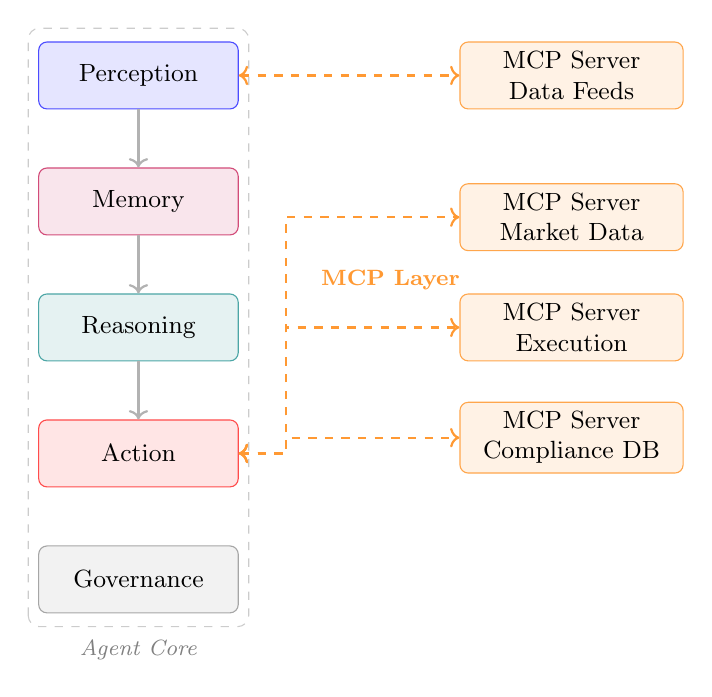
\begin{tikzpicture}[
  mod/.style={
    rectangle,
    rounded corners=3pt,
    draw=#1!70,
    fill=#1!10,
    minimum width=2.5cm,
    minimum height=0.85cm,
    text width=2.3cm,
    align=center,
    font=\small
  },
  server/.style={
    rectangle,
    rounded corners=3pt,
    draw=orange!70,
    fill=orange!10,
    minimum width=2.8cm,
    minimum height=0.85cm,
    text width=2.6cm,
    align=center,
    font=\small
  },
  inarr/.style={->, thick, gray!60},
  mcparr/.style={<->, thick, orange!80, dashed}
]
\node[mod=blue]   (perc) at (0,  5.0) {Perception};
\node[mod=purple] (mem)  at (0,  3.4) {Memory};
\node[mod=teal]   (reas) at (0,  1.8) {Reasoning};
\node[mod=red]    (act)  at (0,  0.2) {Action};
\node[mod=gray]   (gov)  at (0, -1.4) {Governance};
\draw[inarr] (perc) -- (mem);
\draw[inarr] (mem)  -- (reas);
\draw[inarr] (reas) -- (act);
% MCP Servers connected to Perception
\node[server] (s0) at (5.5, 5.0) {MCP Server\\Data Feeds};
\draw[mcparr] (perc.east) -- ++(0.6, 0) |- (s0.west);
% MCP Servers connected to Action
\node[server] (s1) at (5.5, 3.2) {MCP Server\\Market Data};
\node[server] (s2) at (5.5, 1.8) {MCP Server\\Execution};
\node[server] (s3) at (5.5, 0.4) {MCP Server\\Compliance DB};
\draw[mcparr] (act.east) -- ++(0.6, 0) |- (s1.west);
\draw[mcparr] (act.east) -- ++(0.6, 0) |- (s2.west);
\draw[mcparr] (act.east) -- ++(0.6, 0) |- (s3.west);
\node[font=\footnotesize\bfseries, orange!80] at (3.2, 2.4) {MCP Layer};
\draw[dashed, gray!40, rounded corners] (-1.4, -2.0) rectangle (1.4, 5.6);
\node[font=\footnotesize\itshape, gray] at (0, -2.3) {Agent Core};
\end{tikzpicture}
\caption{MCP within the five-module agent architecture. The MCP layer bridges both the perception and action modules with external systems. Perception ingests real-time data via MCP-compliant feed servers, while the action module invokes execution, market data, and compliance services---all without embedding provider-specific logic in the agent core.}
\label{fig:mcp-in-agent}
\end{figure}

\subsubsection{MCP in Financial Services}
The financial services industry is a particularly strong fit for MCP for three reasons. First, financial institutions maintain numerous internal and external data sources, such as trading systems, risk engines, compliance databases, client records, and regulatory portals, making the N$\times$M integration problem especially acute. Second, the industry's strict regulatory requirements demand that every action taken by an AI agent be traceable and attributable to a specific call on a specific system at a specific time; MCP's structured request-response model supports this auditability directly. Third, financial data systems are frequently operated by third-party vendors who can publish MCP-compliant servers as a standard interface, reducing the integration burden on deploying institutions.

The three MCP primitives map naturally onto concrete financial workflows:

\begin{itemize}
  \item \textbf{Resources} supply the read-only context that agents need before acting.
  \begin{itemize}
    \item \textit{Portfolio Management:} the agent retrieves live  Net Asset Value (NAV), position data, and benchmark weights before executing a rebalancing decision.
    \item \textit{Credit Analysis:} the agent pulls a borrower's audited financials, credit history, and sector benchmarks from a document archive to support underwriting.
  \end{itemize}

  \item \textbf{Tools} allow the agent to invoke external systems and trigger actions with real-world consequences.
  \begin{itemize}
    \item \textit{Trade Execution:} the agent submits a limit order to an execution server and receives a structured fill confirmation in return.
    \item \textit{Compliance Monitoring:} the agent calls a sanctions-screening server to check a counterparty against the OFAC list before authorizing a payment.
    \item \textit{Regulatory Reporting:} the agent files a report through a regulatory portal server and receives a submission receipt.
  \end{itemize}

  \item \textbf{Prompts} standardize the agent's communication with stakeholders.
  \begin{itemize}
    \item \textit{Client Advisory:} a reusable prompt template ensures all client-facing summaries conform to the institution's approved communication format and regulatory disclosure standards.
  \end{itemize}
\end{itemize}
% \subsubsection{Security Considerations}

% Because MCP tools represent arbitrary code execution, security is a first-order concern. Three risks warrant specific attention.

% \textbf{Prompt injection through external content.} When an agent retrieves a resource through MCP, that content enters the agent's context window. A malicious actor could embed hidden instructions inside a news article or regulatory filing, attempting to redirect the agent's behavior. All externally retrieved content must be treated as untrusted and filtered before it influences the agent's reasoning.

% \textbf{Tool permission scope.} MCP servers should expose only the permissions required for the task at hand, a principle of \textit{least privilege}. An agent performing read-only market data retrieval should not hold credentials that also allow it to execute trades, since overly permissive servers can be exploited to chain together actions with unintended consequences.

% \textbf{Server authentication.} In production financial deployments, the agent must verify it is communicating with a legitimate MCP server. The MCP specification's OAuth 2.0-based authorization framework, introduced in 2025, addresses this by treating MCP servers as OAuth Resource Servers, enabling token-based authentication scoped to specific servers.

% ----------------------------------------------------------------
\subsection{Multi-Agent Systems}
\label{sec:mas}

Single-agent architectures are powerful for bounded, well-defined tasks. However, many real-world financial problems are too complex, too broad, or too time-critical for any single agent to handle alone. Consider what a bank actually does when it onboards a new corporate client: it must simultaneously verify the client's legal identity, assess its credit risk, check it against sanctions and anti-money-laundering databases, evaluate its product suitability, and prepare a relationship summary for the account manager. A single agent cannot specialize across all of these domains at once.

A \textbf{multi-agent system (MAS)} is a collection of autonomous AI agents that collaborate to accomplish tasks that exceed the capacity of any individual agent \cite{wooldridge2009introduction}. Each agent specializes in a specific function, and together they produce outputs that are richer, faster, and more robust than any single generalist agent could achieve. The case for multi-agent architectures rests on four practical advantages. 
\begin{itemize}
    \item \textbf{Specialization} allows each agent to be optimized for its own domain: a credit agent trained on loan data, a compliance agent trained on regulatory texts, and a market agent trained on price time-series.     
    \item \textbf{Parallelism} removes sequential bottlenecks: if onboarding requires credit assessment, sanctions screening, and product suitability review, a multi-agent system can run all three concurrently, reducing end-to-end latency by an order of magnitude. 
    \item \textbf{Resilience} means that the failure of one specialist agent can be isolated while other agents continue operating. 
    \item \textbf{Scalability} allows new specialist agents to be added without restructuring existing ones: adding a new regulatory jurisdiction requires building a single new compliance agent rather than retraining a monolithic system.
\end{itemize}

\subsubsection{Architectures of Multi-Agent Systems}

The internal structure of a MAS determines how agents communicate, who makes final decisions, and how work is divided. Three principal architectures are used in practice \cite{guo2024large}, illustrated in Figure~\ref{fig:mas-architectures}.

\begin{figure}[h!]
\centering
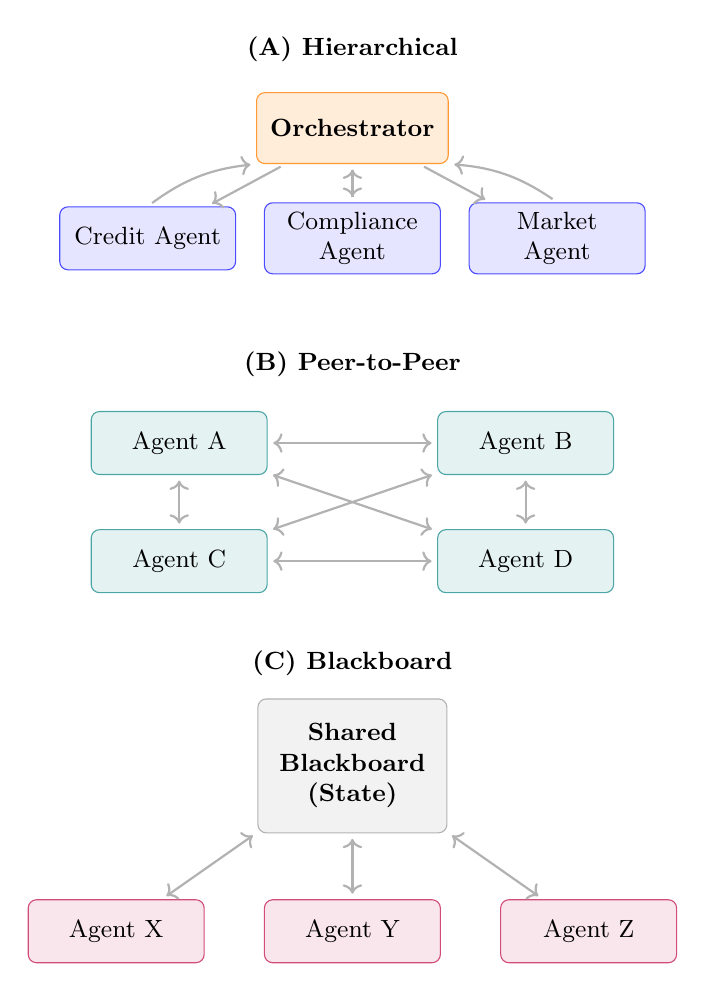
\begin{tikzpicture}[
  agent/.style={
    rectangle,
    rounded corners=3pt,
    draw=#1!70,
    fill=#1!10,
    minimum width=2.2cm,
    minimum height=0.8cm,
    text width=2.0cm,
    align=center,
    font=\small
  },
  orch/.style={
    rectangle,
    rounded corners=3pt,
    draw=orange!80,
    fill=orange!15,
    minimum width=2.4cm,
    minimum height=0.9cm,
    text width=2.2cm,
    align=center,
    font=\small\bfseries
  },
  arr/.style={->, thick, gray!60, shorten >=2pt, shorten <=2pt},
  biarr/.style={<->, thick, gray!60, shorten >=2pt, shorten <=2pt}
]

% ===================== (A) Hierarchical =====================
\node[font=\bfseries\small] at (0, 6.6) {(A) Hierarchical};

\node[orch]       (orch) at (0, 5.6) {Orchestrator};
\node[agent=blue] (a1)   at (-2.6, 4.2) {Credit Agent};
\node[agent=blue] (a2)   at (0.0, 4.2) {Compliance\\Agent};
\node[agent=blue] (a3)   at (2.6, 4.2) {Market\\Agent};

\draw[arr] (orch) -- (a1);
\draw[arr] (orch) -- (a2);
\draw[arr] (orch) -- (a3);
\draw[arr] (a1.north) to[bend left=15] (orch.south west);
\draw[arr] (a2) -- (orch);
\draw[arr] (a3.north) to[bend right=15] (orch.south east);

% ===================== (B) Peer-to-Peer =====================
\node[font=\bfseries\small] at (0, 2.6) {(B) Peer-to-Peer};

\node[agent=teal] (p1) at (-2.2, 1.6) {Agent A};
\node[agent=teal] (p2) at ( 2.2, 1.6) {Agent B};
\node[agent=teal] (p3) at (-2.2, 0.1) {Agent C};
\node[agent=teal] (p4) at ( 2.2, 0.1) {Agent D};

\draw[biarr] (p1) -- (p2);
\draw[biarr] (p1) -- (p3);
\draw[biarr] (p2) -- (p4);
\draw[biarr] (p3) -- (p4);
\draw[biarr] (p1) -- (p4);
\draw[biarr] (p2) -- (p3);

% ===================== (C) Blackboard =====================
\node[font=\bfseries\small] at (0, -1.2) {(C) Blackboard};

\node[
  draw=gray!60,
  fill=gray!10,
  minimum width=2.4cm,
  minimum height=1.7cm,
  rounded corners=3pt,
  font=\small\bfseries,
  align=center
] (bb) at (0, -2.5) {Shared\\Blackboard\\(State)};

\node[agent=purple] (b1) at (-3.0, -4.6) {Agent X};
\node[agent=purple] (b2) at ( 0.0, -4.6) {Agent Y};
\node[agent=purple] (b3) at ( 3.0, -4.6) {Agent Z};

\draw[biarr] (b1) -- (bb);
\draw[biarr] (b2) -- (bb);
\draw[biarr] (b3) -- (bb);

\end{tikzpicture}
\caption{Three principal multi-agent architectures. (A) In the hierarchical architecture, an orchestrator agent decomposes tasks and delegates to specialists who report results back up. (B) In the peer-to-peer architecture, agents communicate directly without a central coordinator. (C) In the blackboard architecture, agents coordinate indirectly by reading from and writing to a shared state.}
\label{fig:mas-architectures}
\end{figure}

In a \textbf{hierarchical} (orchestrator-worker) architecture, one agent decomposes a high-level goal into subtasks, assigns those subtasks to specialist worker agents, and integrates their outputs into a final result \cite{guo2024large}. This mirrors the role of a senior analyst who coordinates a deal team: she does not personally model the target company's financials or conduct the legal review, but divides the work, sets deadlines, and assembles the final report. A loan origination system built this way might have an orchestrator that assigns document parsing, credit scoring, sanctions screening, collateral valuation, and report formatting to a dedicated specialist agent.

In a \textbf{peer-to-peer} architecture, there is no central orchestrator: agents communicate directly with each other, negotiating task assignments on a bilateral basis \cite{wooldridge2009introduction}. This architecture is more resilient, but requires careful design to prevent coordination failures or conflicting actions. It suits decentralized financial environments such as inter-bank settlement networks, where agents representing different institutions must coordinate without any single institution acting as a central authority.

In a \textbf{blackboard} architecture, all agents share access to a common state store from which they read inputs and to which they write outputs \cite{craig1988blackboard}. Agents coordinate indirectly by observing and updating the shared state. This is well-suited to financial risk management, where specialist agents for market risk, credit risk, liquidity risk, and operational risk each contribute assessments to a shared risk dashboard. Every state change is recorded, providing a natural audit trail of the system's collective reasoning.

Table~\ref{tab:mas-architecture-comparison} summarizes the trade-offs between these architectures.

\begin{table}[h!]
\centering
\caption{Comparison of Multi-Agent System Architectures for Financial Applications.}
\label{tab:mas-architecture-comparison}
\renewcommand{\arraystretch}{1.3}
\begin{tabular}{|p{2.5cm}|p{2.8cm}|p{2.8cm}|p{2.9cm}|}
\hline
\textbf{Architecture} & \textbf{Key Advantage} & \textbf{Key Limitation} & \textbf{Financial Use Case} \\
\hline
\textbf{Hierarchical} & Clear accountability; easy to audit and govern & Orchestrator is a single point of failure & Loan origination, M\&A due diligence, client onboarding \\
\hline
\textbf{Peer-to-Peer} & Resilient; no central bottleneck & Coordination complexity; risk of conflicting actions & Inter-bank settlement, FX netting, consortium credit decisions \\
\hline
\textbf{Blackboard} & Natural audit trail; indirect coordination reduces coupling & Shared state requires robust concurrency controls & Risk aggregation dashboards, regulatory reporting pipelines \\
\hline
\end{tabular}
\end{table}

\subsubsection{Coordination Patterns}

Within any architecture, agents must coordinate their work through two fundamental patterns. \textbf{Sequential chaining} passes the output of one agent as the input to the next, forming a pipeline. In a trade surveillance pipeline, a data-cleaning agent processes raw tick data, passes it to a pattern-detection agent, which flags anomalies for a regulatory-assessment agent, which drafts reports for a human reviewer. Each stage depends on the previous one, making the pipeline predictable and auditable.

\textbf{Parallel fan-out with aggregation} dispatches the same input to multiple agents simultaneously and then synthesizes their independent outputs. In a credit committee scenario, the same loan application might be sent concurrently to a quantitative credit model agent, a qualitative management assessment agent, and a sector-outlook agent. An aggregator agent then synthesizes the three assessments into a committee-ready memo. Complex financial workflows typically combine both patterns: sequential stages where outputs genuinely depend on earlier results, and parallel stages where independent analyses can run concurrently.

% ----------------------------------------------------------------
\subsubsection{The Agent2Agent Protocol}
\label{sec:a2a}

Multi-agent systems work well when all agents are built by the same team, using the same framework, and running on the same platform. In the real world of financial services, this assumption rarely holds. A bank might deploy credit agents built with one framework, compliance agents from a regtech vendor using a different framework, trading agents from a third-party platform, and client-advisory agents from yet another provider. Making them collaborate requires every pair of agents to agree on a custom integration, recreating the same N$\times$M fragmentation problem that MCP solved at the agent-to-tool level.

The \textbf{Agent2Agent (A2A) Protocol} solves this problem. It is an open communication standard that enables AI agents to discover each other, exchange information, and coordinate tasks regardless of which framework they were built with or which vendor operates them \cite{googlea2a2025}. Introduced by Google in April 2025, it was donated to the Linux Foundation in June 2025 and is now maintained as a vendor-neutral open standard.

The distinction between MCP and A2A is precise and important. MCP governs the relationship between an agent and its \textit{tools}: how an agent calls an API, retrieves a document, or executes a function. A2A governs the relationship between an \textit{agent and another agent}: how one autonomous reasoner delegates work to, and receives results from, another autonomous reasoner \cite{googlea2a2025}. A tool has fixed, structured input-output behavior. An agent can exercise judgment, ask clarifying questions, decompose tasks further, and return results in open-ended form.

A practical analogy from financial institutions makes this distinction clear. MCP is the set of standardized terminals and interfaces through which staff access systems: the Bloomberg terminal, the risk management dashboard, and the regulatory portal. A2A is the set of protocols through which staff communicate with each other: the format of a credit memo, the procedure for escalating a risk limit breach, and the workflow for routing an unusual transaction for senior review. Both are essential; neither substitutes for the other.

% \subsubsection{Core A2A Concepts}

% A2A defines a small set of concepts that together cover the full lifecycle of inter-agent collaboration.

% Before two agents can collaborate, they must understand what each other is capable of. A2A addresses this through the \textbf{Agent Card}: a structured JSON document that each agent publishes at a well-known URL endpoint, advertising its identity, capabilities, and communication preferences \cite{googlea2a2025}. An Agent Card is the agent equivalent of a professional business card combined with a job description. A compliance screening agent, for example, might specify: the tasks it can perform (OFAC screening, PEP checks, AML pattern detection), the input formats it accepts (structured transaction records, free-text client names), the output formats it produces (JSON risk assessments, plain-language explanations), and its authentication requirements.

% The central unit of work is the \textbf{Task}: a structured object representing a request from a client agent to a server agent, with a unique identifier and a status that progresses through defined states \cite{googlea2a2025}. Tasks support two execution modes. Synchronous tasks complete immediately. Asynchronous tasks are long-running: the server agent accepts the task, begins processing, and notifies the client of progress through streaming updates or push notifications. This is critical for financial applications where operations such as a complex credit analysis or a large-scale transaction monitoring sweep may take minutes or hours to complete. The deliverable produced by a completed task is called an \textbf{Artifact}: a structured data object, a formatted document, a risk score, or any other result type.

% Agents exchange structured \textbf{Messages} composed of one or more \textbf{Parts}, where each Part carries a specific content type: plain text, structured data, a file, or an embedded function call \cite{googlea2a2025}. This multi-part design allows a single message to combine a natural-language instruction with a structured data payload, for example, a portfolio rebalancing instruction accompanied by the current holdings in JSON format.

% \subsubsection{The A2A Communication Lifecycle}

% Figure~\ref{fig:a2a-lifecycle} illustrates the full lifecycle of a task exchange between two A2A agents.

% \begin{figure}[h!]
% \centering
% \begin{tikzpicture}[
%   box/.style={
%     rectangle,
%     rounded corners=3pt,
%     draw=#1!70,
%     fill=#1!10,
%     minimum width=3.2cm,
%     minimum height=0.85cm,
%     text width=3.0cm,
%     align=center,
%     font=\small
%   },
%   step/.style={
%     rectangle,
%     rounded corners=2pt,
%     draw=gray!50,
%     fill=gray!8,
%     minimum width=3.6cm,
%     minimum height=0.75cm,
%     text width=3.4cm,
%     align=center,
%     font=\footnotesize
%   },
%   arr/.style={->, thick, gray!60, shorten >=2pt, shorten <=2pt}
% ]

% % Columns
% \node[box=blue] (client) at (0, 7.5) {\textbf{Client Agent}\\(Orchestrator)};
% \node[box=green!60!black] (server) at (8.0, 7.5) {\textbf{Server Agent}\\(Specialist)};

% \draw[dashed, gray!40] (0, 7.0) -- (0, -0.5);
% \draw[dashed, gray!40] (8.0, 7.0) -- (8.0, -0.5);

% % Step 1: Discovery
% \node[step] (d1) at (0, 6.2) {1. Fetch Agent Card};
% \node[step] (d2) at (8.0, 6.2) {Publish Agent Card};
% \draw[arr] (d1) -- node[above, font=\footnotesize]{GET /.well-known/agent-card} (d2);

% % Step 2: Task creation
% \node[step] (t1) at (0, 5.0) {2. Create Task \& send first message};
% \node[step] (t2) at (8.0, 5.0) {Receive task; begin processing};
% \draw[arr] (t1) -- node[above, font=\footnotesize]{POST /tasks (JSON-RPC)} (t2);

% % Step 3: Multi-turn interaction
% \node[step] (m1) at (8.0, 3.8) {3. Request clarification\\or more context};
% \node[step] (m2) at (0, 3.8) {Provide additional input};
% \draw[arr] (m1) -- node[above, font=\footnotesize]{message: \{parts\}} (m2);
% \draw[arr] (m2) -- node[below, font=\footnotesize]{message: \{parts\}} (m1);

% % Step 4: Progress updates
% \node[step] (p1) at (8.0, 2.6) {4. Stream progress updates};
% \node[step] (p2) at (0, 2.6) {Monitor task status};
% \draw[arr] (p1) -- node[above, font=\footnotesize]{SSE / push notification} (p2);

% % Step 5: Artifact delivery
% \node[step] (a1) at (8.0, 1.4) {5. Deliver Artifact\\(task complete)};
% \node[step] (a2) at (0, 1.4) {Receive \& integrate result};
% \draw[arr] (a1) -- node[above, font=\footnotesize]{artifact: \{type, content\}} (a2);

% % Step 6: Governance log
% \node[step, draw=orange!60, fill=orange!8] (g1) at (0, 0.2) {6. Log to audit trail};
% \node[step, draw=orange!60, fill=orange!8] (g2) at (8.0, 0.2) {6. Log to audit trail};

% \end{tikzpicture}
% \caption{The A2A task lifecycle between a client agent and a server agent. Discovery via the Agent Card is followed by task creation, optional multi-turn clarification, asynchronous progress updates, and final artifact delivery. Both agents log all interactions to their audit trails for governance and regulatory purposes.}
% \label{fig:a2a-lifecycle}
% \end{figure}

% The lifecycle proceeds through five stages. First, the client agent fetches the server agent's Agent Card to confirm its capabilities. Second, the client creates a Task and sends it with an initial message. Third, if the server agent needs additional context, for example, a compliance agent that requires a client's country of residence before determining which regulatory framework applies, it sends clarifying messages back to the client in a genuinely bi-directional exchange. Fourth, for long-running tasks, the server streams progress updates. Fifth, when processing is complete, the server delivers the Artifact. Both agents record the full interaction in their audit logs, satisfying the traceability requirements of regulated financial environments.

% \subsubsection{MCP and A2A Together}

% A2A and MCP address different layers of the same challenge and are designed to be used together. The recommended pattern is: agents use MCP to interact with tools and data sources, and A2A to interact with other agents \cite{googlea2a2025}. Figure~\ref{fig:a2a-mcp-layers} illustrates how these two protocols form complementary layers within a unified agent architecture.

% \begin{figure}[h!]
% \centering
% \begin{tikzpicture}[
%   layer/.style={
%     rectangle,
%     rounded corners=4pt,
%     draw=#1!70,
%     fill=#1!10,
%     minimum width=10cm,
%     minimum height=1.1cm,
%     text width=9.8cm,
%     align=center,
%     font=\small
%   }
% ]
% \node[layer=blue] (agents) at (5.5, 3.2) {\textbf{Agent Layer}\quad Agents reason, plan, and collaborate\quad \textit{coordinated via A2A}};
% \node[layer=orange] (mcp) at (5.5, 1.9) {\textbf{Tool and Data Layer}\quad APIs, databases, execution systems, document stores\quad \textit{accessed via MCP}};
% \node[layer=gray] (infra) at (5.5, 0.6) {\textbf{Infrastructure Layer}\quad HTTP, JSON-RPC 2.0, OAuth 2.0, Server-Sent Events};

% \draw[->, thick, gray!60] (agents.south) -- (mcp.north);
% \draw[->, thick, gray!60] (mcp.south) -- (infra.north);

% \end{tikzpicture}
% \caption{A2A and MCP as complementary protocol layers. A2A operates between agents at the collaboration layer; MCP operates between an agent and its tools at the integration layer. Both are built on the same underlying web standards.}
% \label{fig:a2a-mcp-layers}
% \end{figure}

% A concrete financial example illustrates how the two protocols interlock. A corporate client onboarding system deploys four agents: an orchestrator agent, a document-processing agent, a KYC compliance agent, and a credit assessment agent. The orchestrator uses A2A to delegate tasks to the other three agents. Each specialist agent, in turn, uses MCP to call the tools it needs: the document-processing agent calls an OCR server; the KYC agent calls a sanctions database server; the credit agent calls a financial data API. The A2A layer handles agent-to-agent coordination; the MCP layer handles agent-to-tool integration. The two protocols do not overlap or conflict.

% Table~\ref{tab:a2a-finance-use-cases} maps A2A-enabled multi-agent workflows to concrete financial applications.

% \begin{table}[h!]
% \centering
% \caption{A2A-Enabled Multi-Agent Workflows in Financial Services.}
% \label{tab:a2a-finance-use-cases}
% \renewcommand{\arraystretch}{1.3}
% \begin{tabular}{|p{2.5cm}|p{3.5cm}|p{5.0cm}|}
% \hline
% \textbf{Domain} & \textbf{Agents Involved} & \textbf{A2A Coordination Pattern} \\
% \hline
% Corporate Onboarding & Orchestrator, Document, KYC, Credit, Reporting & Orchestrator fans out subtasks in parallel; aggregates outputs into onboarding decision memo \\
% \hline
% Trade Surveillance & Market data agent, Pattern detection agent, Regulatory filing agent & Sequential pipeline: each stage consumes the prior agent's artifact \\
% \hline
% Portfolio Management & Research agent, Risk agent, Execution agent & Research and risk agents run in parallel; execution agent waits for both before acting \\
% \hline
% Loan Origination & Application parser, Credit scorer, Valuation agent, Compliance screener & Orchestrator coordinates four specialist agents; escalates borderline cases to a human reviewer \\
% \hline
% Regulatory Reporting & Data extraction agent, Reconciliation agent, Filing agent & Sequential pipeline with blackboard shared state for audit trail \\
% \hline
% \end{tabular}
% \end{table}

% \subsection{Governance of Multi-Agent Systems}

% Four risks are specific to environments where multiple autonomous agents interact.

% \textbf{Emergent behavior.} When agents interact, their collective behavior can differ from the behavior of any individual agent in isolation. The 2010 Flash Crash is the canonical example: algorithmic trading systems interacting at high speed produced a self-reinforcing feedback loop that temporarily erased nearly \$1 trillion in market value, even though each individual system was operating within its own design parameters \cite{kirilenko2017flash}. Multi-agent financial systems face an analogous risk; individually well-governed agents can produce unanticipated collective decisions if their interactions are not carefully designed and tested.

% \textbf{Accountability propagation.} When a multi-agent pipeline produces a consequential output, such as a credit decision, a trade, or a regulatory filing, it can be difficult to determine which agent in the chain is responsible for an error. A2A's audit logging requirement, combined with each agent's internal governance layer, provides a chain of custody for every decision: each agent records the tasks it received, the tools it called, and the artifacts it produced.

% \textbf{Trust between agents.} In a system where agents from different vendors interact, a client agent cannot assume that a server agent is behaving honestly or within its declared capabilities. A2A addresses this through signed Agent Cards, allowing clients to cryptographically verify the identity and declared capabilities of a server agent before delegating sensitive tasks.

% \textbf{Cascading failures.} If one agent in a pipeline produces an incorrect output and downstream agents treat it as ground truth, the error can propagate and amplify through the system. Robust multi-agent governance implements validation checkpoints between pipeline stages, where anomalous outputs trigger human-in-the-loop review rather than automatic downstream processing.

\section{Use Cases}

% ------------------------------------------------------------------
% \begin{usecasebox}{JPMorgan Chase: LLM Suite and the Agentic Enterprise}
% JPMorgan Chase, the world's largest bank by market capitalisation, is pursuing what its Chief Analytics Officer Derek Waldron describes as the goal of becoming \emph{``a fully AI-connected enterprise''}: every employee equipped with a personalised AI assistant, every back-office process automated by AI agents, and every client experience curated by an AI concierge \cite{jpmorgan_cnbc2025}. The centrepiece of this transformation is \textbf{LLM Suite}, a proprietary portal that provides secure, firewalled access to large language models from OpenAI and Anthropic across the bank's business lines. Developed entirely in-house and updated every eight weeks as additional internal data sources and applications are connected, the platform earned American Banker's \emph{Innovation of the Year} award for 2025 \cite{jpmorgan_ab2025}.

% By late 2025, approximately 250{,}000 employees had access to LLM Suite, with roughly half using it daily. In a live demonstration for CNBC — the first ever granted to an outside journalist — Waldron prompted the system to prepare a five-page investment banking presentation for a meeting with Nvidia's leadership. The platform produced a credible, formatted deck in approximately 30 seconds, work that would previously have required a team of junior analysts working through the night \cite{jpmorgan_cnbc2025}.

% JPMorgan is now in the next phase of its AI blueprint: deploying \textbf{agentic AI} for multi-step tasks. Key capabilities in production or advanced development include:

% \begin{itemize}
%     \item Agentic generation of investment banking pitch books and confidential information memoranda, compressing work that previously spanned days for analyst teams into minutes.
%     \item AI drafting of credit risk memos, with one US bank deploying a similar workflow reporting a 20--60\% increase in analyst productivity and a 30\% improvement in credit turnaround time \cite{neurons_lab2026}.
%     \item Client advisory agents that improve response times during market volatility and contribute to measurable increases in gross sales within asset and wealth management.
%     \item Tiered governance enforced through the LLM Suite architecture, which maintains data residency within JPMorgan's own infrastructure, preventing proprietary information from leaving the bank's perimeter.
% \end{itemize}

% The deployment illustrates a central governance principle from Section 3.5: building the safety and oversight infrastructure before extending agent autonomy, not retrofitting it afterward. As Waldron acknowledges, a significant \emph{``value gap''} still exists between what the technology is capable of and the ability of the enterprise to fully capture that value — a gap the bank is closing by connecting thousands of internal applications into a coherent, AI-consumable ecosystem \cite{jpmorgan_cnbc2025}.
% \end{usecasebox}

% ------------------------------------------------------------------
% \begin{usecasebox}{Mastercard: Agent Pay and the Infrastructure of Agentic Commerce}
% In April 2025, Mastercard launched \textbf{Agent Pay}, its Agentic Payments Programme, making it one of the first global payment networks to build dedicated infrastructure for a world in which AI agents transact autonomously on behalf of consumers and businesses \cite{mastercard_agentpay2025}. The programme is a direct response to a structural shift in commerce: consumers are increasingly turning to conversational AI platforms for product discovery and purchasing, and an autonomous agent that can \emph{recommend} a product must also be able to \emph{pay} for it securely and transparently.

% The technical foundation of Agent Pay is \textbf{Mastercard Agentic Tokens} — dynamic digital credentials that extend the bank's proven tokenisation technology (which already underlies contactless payments and secure card-on-file) into agentic commerce. Agentic tokens work as follows:

% \begin{itemize}
%     \item Only registered and verified AI agents may obtain agentic tokens, ensuring that every transaction can be traced to an authorised, identified agent rather than an anonymous or potentially malicious script.
%     \item Each token encodes consumer-defined spending limits and permission scopes, so the agent can only act within boundaries the cardholder has explicitly set.
%     \item Every transaction is cryptographically linked to the specific authorised interaction, providing a complete, tamper-evident audit trail for dispute resolution and fraud investigation.
%     \item Mastercard's existing fraud prevention and biometric authentication layers extend seamlessly to agentic transactions, with no new technical requirements for merchants.
% \end{itemize}

% By October 2025, Mastercard had partnered with PayPal to integrate Agent Pay into PayPal's wallet, giving hundreds of millions of consumers and tens of millions of merchants access to agent-driven commerce without complex implementation \cite{mastercard_paypal2025}. Collaborations with Microsoft (Azure OpenAI Service, Copilot Studio), Google, Stripe, Ant International, and Cloudflare — the latter for cryptographic agent-identity verification via the Web Bot Authentication standard — extended Agent Pay's reach across the global payments ecosystem. By November 2025, all US Mastercard cardholders were enabled for Agent Pay-powered transactions, with global rollout following shortly thereafter.

% From the perspective of Chapter 5, Agent Pay exemplifies the \textbf{action module} and \textbf{governance layer} working in concert: agentic tokens are the mechanism by which an agent's payment action is executed (action module), while the registration, permission scope, and audit trail architecture enforce the consumer's intent and provide the traceability required for regulated financial activity (governance layer).
% \end{usecasebox}

% ------------------------------------------------------------------
\begin{usecasebox}{HSBC: AML AI and the Dynamic Risk Assessment System}
HSBC, one of the world's largest banking organisations, processes an average of 1.2 billion transactions per month that must be screened for signs of financial crime \cite{google_hsbc_aml}. For years, HSBC — like most large banks — relied on rules-based transaction monitoring: compliance teams manually specified which patterns the system should flag. This approach generated an overwhelming volume of false positives, with over 95\% of flagged transactions ultimately found to be legitimate, creating enormous investigative backlogs and delaying the detection of genuinely suspicious activity \cite{google_hsbc_aml}.

To address this challenge, HSBC partnered with Google Cloud to co-develop \textbf{AML AI}, a machine-learning-powered agent system deployed as its primary transaction monitoring infrastructure under the name \textbf{Dynamic Risk Assessment (DRA)}. Unlike its rules-based predecessor, AML AI:

\begin{itemize}
    \item Learns directly from HSBC's vast global transaction data rather than from manually specified rules, enabling it to detect novel laundering patterns that no analyst has yet thought to specify.
    \item Creates dynamic, continuously updated risk scores for customers by analysing transaction patterns, network behaviours, and KYC data simultaneously, rather than evaluating transactions in isolation.
    \item Provides explainable outputs that compliance investigators can interpret and present to regulators, satisfying the \emph{right to explanation} requirements.
    \item Identifies two to four times as much genuine suspicious activity as the previous rules-based system, while simultaneously reducing the total volume of alerts by 60\%, allowing investigators to concentrate effort on cases that truly warrant it \cite{google_hsbc_aml}.
\end{itemize}

The operational results were transformative: HSBC reported twice as much confirmed financial crime identified in commercial banking and almost four times as much in retail banking following deployment. The system has since been expanded from its initial UK and Hong Kong markets to additional regions, and HSBC received the Celent Model Risk Manager of the Year award for 2023 in recognition of the innovation. In 2025, HSBC announced a major reorganisation explicitly designed to accelerate further investment in generative AI and machine learning across its Corporate and Institutional Banking division \cite{klover_hsbc2025}.

% The HSBC case study is significant for two reasons beyond its headline metrics. First, it demonstrates the \textbf{perception module} operating at financial-institution scale: an agent that continuously ingests and semantically grounds a billion-plus monthly transactions across dozens of jurisdictions, extracting structured risk signals from inherently noisy data. Second, it illustrates the governance principle that explainability must be engineered from the outset: the decision to produce interpretable risk scores was a design choice, not a post-hoc addition, and it is precisely what made the system viable in a regulated environment.
\end{usecasebox}

% ------------------------------------------------------------------
\begin{usecasebox}{Morgan Stanley: AI-powered “super agents”}

Morgan Stanley has developed a suite of \textbf{AI-powered “super agents”} designed to function as digital coworkers capable of planning and executing complex, multi-step financial tasks. These agents are inspired by J.A.R.V.I.S., the fictional AI assistant, with the goal of enabling financial advisors to direct work without performing all underlying tasks themselves \cite{finplanning_mswm2025}.

The system is organized into three primary functional areas. The \textit{Branch Operations Companion} acts as a support tool for client service associates, performing actions beyond simple information retrieval, including moving money, changing beneficiaries, and opening accounts. The \textit{Portfolio-Building Agent} assists in constructing customized portfolios for new clients based on constraints such as asset allocation, expenses, and available investment options, and can implement these plans once approved by an advisor. The \textit{Client Service Agent} provides continuous interaction by responding to client requests, such as reporting account balances and sending tax documents, with plans to expand into additional services as risks are addressed.

These agents are designed to handle multi-step workflows, combining planning and execution capabilities within financial processes. A key principle of the system is the \textbf{human-in-the-loop} approach, where financial advisors retain the final decision-making authority over all AI-generated recommendations and actions.

\begin{itemize}
  \item Improved \textbf{operational efficiency}, as agents automate routine tasks performed by client service associates.
  \item Enhanced \textbf{portfolio construction}, with agents generating customized investment plans based on defined constraints.
  \item Continuous \textbf{client service}, enabling responses to client requests at any time.
  \item Maintained \textbf{human oversight}, ensuring that all actions and recommendations are reviewed and approved by advisors.
  \item Strengthened \textbf{data reliability and governance}, through the use of proprietary data and internal machine learning systems to ensure accuracy and personalization.
\end{itemize}

The Morgan Stanley case demonstrates the use of AI agents as digital coworkers that support financial professionals by automating execution and assisting in complex workflows, while maintaining human control and compliance within the decision-making process.



% Morgan Stanley Wealth Management oversees more than \$6 trillion in client assets and employs over 16{,}000 financial advisors. Since 2023, the firm has built a suite of AI agent tools under the brand \textbf{AI @ Morgan Stanley}, developed in a strategic partnership with OpenAI — the first such arrangement in the wealth management industry \cite{openai_morganstanley}.

% The suite's evolution illustrates the stepwise expansion of agent autonomy . The first tool, \textbf{AI @ Morgan Stanley Assistant}, deployed in 2023, is an LLM-powered knowledge agent giving advisors natural-language access to more than 100{,}000 proprietary research reports, regulatory documents, and internal memos. Document retrieval efficiency improved from 20\% to 80\%, and over 98\% of advisor teams now use the tool daily \cite{openai_morganstanley}. The second tool, \textbf{AI @ Morgan Stanley Debrief} (launched June 2024 and expanded to the full advisor field in July 2025), transcribes client meetings with consent, extracts action items, and automatically drafts follow-up emails and CRM entries — a multi-step workflow that saves each advisor an estimated 15 hours per week \cite{investmentnews_mswm2025}.

% In 2025 and 2026, Morgan Stanley moved to the next stage: \textbf{AI Super Agents}. As described by Jed Finn, Head of Wealth Management, the firm is building ``super agents'' composed of ``hundreds, if not thousands'' of smaller, specialised sub-agents, designed to take \emph{action} rather than merely retrieve information \cite{finplanning_mswm2025}. Planned capabilities include:

% \begin{itemize}
%     \item A portfolio-building super agent that, given a client's investment objectives, constructs a fully specified portfolio constrained by asset allocation targets, historical performance, expense ratios, and Sharpe ratio requirements, without requiring the advisor to manually evaluate each option.
%     \item An account service super agent that handles routine tasks currently performed by client service associates — account openings, fund transfers, and document requests — freeing human staff for higher-value client interactions.
%     \item A Roth Conversion Analyst agent that automatically pulls client data and provides a structured conversion recommendation when the advisor prompts it with forward-looking assumptions.
% \end{itemize}

% Finn's stated design inspiration is \emph{J.A.R.V.I.S.}, the fictional AI in the Iron Man films: an agent that enables the advisor to ``direct the work, but not have to do the work'' \cite{finplanning_mswm2025}. The architecture directly implements the hierarchical multi-agent pattern from Section 4.3: a top-level orchestrator receives the advisor's high-level objective and fans out sub-tasks to specialist agents, each of which invokes its own tools via MCP-style integrations with execution systems, CRM platforms, and risk engines. Human oversight is preserved at the level of the advisor, who reviews, approves, or redirects agent recommendations before client-facing actions are taken.

\end{usecasebox}

% ------------------------------------------------------------------
\begin{usecasebox}{Use Case: Goldman Sachs AI-Powered Algorithmic Trading}
Goldman Sachs has incorporated advanced machine learning into its trading infrastructure to overcome the limitations of traditional strategies in processing high-frequency financial data. Central to this transformation is the use of \textbf{AI agents} as modular, autonomous components that continuously perceive, analyze, and act on market information in near real time \cite{cnbc_gs2025}. These AI agents operate across the trading lifecycle. 
\begin{itemize}
    \item \textit{Perception agents} ingest structured data such as tick-level prices, order books, and technical indicators, as well as unstructured data through Natural Language Processing (NLP), including financial news and central bank communications. 
    \item \textit{Reasoning agents} process these inputs using statistical learning and reinforcement learning techniques to generate trading signals and evaluate strategies such as momentum, mean-reversion, and arbitrage. 
    \item \textit{Action agents} execute trades, rebalance portfolios, and adjust risk exposures dynamically. This multi-agent architecture enables parallel evaluation of strategies and continuous adaptation to evolving market conditions.
\end{itemize}

A key advantage of this approach is the integration of quantitative and qualitative signals. NLP-based agents extract relevant information from unstructured sources, enriching traditional market data and improving responsiveness to macroeconomic events and sentiment shifts. The interaction between agents creates feedback loops, where execution outcomes inform future decision-making, reflecting a transition from static models to adaptive, agent-based financial systems.

All agents operate within a strict Model Risk Management (MRM) framework, ensuring validation, stress testing, monitoring, and explainability. Each decision is auditable, supporting regulatory compliance and institutional trust. Human traders maintain oversight through monitoring dashboards, with the ability to intervene when necessary.

Overall, the Goldman Sachs case illustrates that AI agents in finance act as \textbf{cognitive multipliers}, augmenting human expertise rather than replacing it. By orchestrating specialized agents across perception, reasoning, and action layers, financial institutions can achieve scalable, adaptive, and robust decision-making while maintaining transparency and governance.


% Goldman Sachs launched the \textbf{GS AI Assistant} in January 2025, initially releasing it to approximately 10{,}000 employees across trading, investment banking, and asset management \cite{cnbc_gs2025}. By June 2025, Chief Information Officer Marco Argenti announced a firm-wide rollout to all 46{,}500 knowledge workers via an internal memo confirmed by Reuters \cite{pymnts_gs_firmwide}. The tool provides a unified, firewalled interface to multiple large language models — including models from OpenAI, Google, Meta, and Anthropic — with role-specific functionality tailored to developers, investment bankers, research analysts, and wealth management staff.

% The assistant's initial scope was deliberately bounded: summarizing lengthy documents, drafting emails, proofreading, and translating code between programming languages. Internal benchmarks reported a 40\% improvement in time-to-deliver for standard coding tasks and an 18\% reduction in routine helpdesk tickets \cite{digitaldefynd_gs2025}. These results established institutional trust in the system before its autonomy was expanded.

% In July 2025, Goldman Sachs announced the launch of a pilot \textbf{autonomous coder agent} — an agentic system capable of executing complex, multi-step software engineering tasks with minimal human supervision \cite{cnbc_gs_coder2025}. Unlike the assistant, which responds to queries, the autonomous coder agent plans a sequence of actions, executes them, observes the results, and iterates — precisely the Perception-Reasoning-Action loop. Argenti described the productivity potential as ``three to four times the rate of previous AI tools'' and characterised the system as a proof point for expanding agentic capabilities to other roles across the bank \cite{cnbc_gs_coder2025}. Goldman's embedded engineers from Anthropic began co-designing autonomous agents for compliance workflows in early 2025, with production deployment of agents for trade accounting, due diligence review, and client onboarding announced in February 2026 \cite{aicerts_gs2026}.

% The governance approach Goldman has adopted is instructive. Human reviewers are maintained throughout the current deployment phase, with employees trained to recognise model errors; the firm tracks ``capacity created'' rather than login metrics, concentrating leadership attention on demonstrable economic value rather than adoption statistics \cite{digitaldefynd_gs2025}. Argenti's framing — a \emph{``hybrid workforce''} where engineers supervise the output of agents rather than performing the underlying tasks themselves — is a practical illustration of the tiered Human-in-the-Loop structure described in Section 3.5: as the autonomous coder demonstrates reliable performance on bounded software tasks, the threshold for unsupervised operation is progressively raised.
\end{usecasebox}


\section{AI Tutorial}
\subsection*{Tutorial: Credit Risk Assessment Agent}

This example constructs a financial agent that evaluates loan applications by computing key credit risk ratios and retrieving sector benchmark data. The agent demonstrates how the ReAct reasoning pattern naturally decomposes a multi-step underwriting task: it first computes the applicant's financial ratios, then retrieves the relevant industry benchmarks, and finally synthesises both into a structured credit assessment. This mirrors the workflow of a junior credit analyst, but executes in seconds across any number of applications.

The agent illustrates a core principle of financial AI design: separating \textit{computation} (ratio calculation) from \textit{knowledge retrieval} (benchmark lookup) into distinct tools allows the reasoning engine to invoke each capability precisely when needed, producing a transparent and auditable decision trace.

\begin{minted}{python}
import warnings
from langgraph.warnings import LangGraphDeprecatedSinceV10
warnings.filterwarnings("ignore", category=LangGraphDeprecatedSinceV10)

from langchain_openai import ChatOpenAI
from langgraph.prebuilt import create_react_agent
from langchain_core.tools import tool

# Step 1: Initialize the LLM
llm = ChatOpenAI(model="gpt-5", temperature=0)

# Step 2: Define credit analysis tools

@tool
def compute_financial_ratios(
    annual_income: float,
    total_debt: float,
    monthly_expenses: float,
    loan_amount: float,
    loan_term_years: int,
    interest_rate: float
) -> str:
    """Compute key credit risk ratios for a loan applicant.
    Returns debt-to-income ratio, loan-to-income ratio,
    and estimated monthly payment coverage ratio.
    All monetary inputs should be in the same currency."""
    try:
        # Debt-to-Income ratio (DTI)
        monthly_income = annual_income / 12
        dti = (total_debt / annual_income) * 100

        # Loan-to-Income ratio (LTI)
        lti = loan_amount / annual_income

        # Monthly payment estimate (standard amortisation)
        monthly_rate = interest_rate / 100 / 12
        n_payments = loan_term_years * 12
        if monthly_rate > 0:
            monthly_payment = loan_amount * (
                monthly_rate * (1 + monthly_rate) ** n_payments
            ) / ((1 + monthly_rate) ** n_payments - 1)
        else:
            monthly_payment = loan_amount / n_payments

        # Payment Coverage Ratio: disposable income vs. payment
        disposable_income = monthly_income - monthly_expenses
        coverage_ratio = disposable_income / monthly_payment

        return (
            f"Debt-to-Income (DTI): {dti:.1f}%\n"
            f"Loan-to-Income (LTI): {lti:.2f}x\n"
            f"Estimated Monthly Payment: ${monthly_payment:,.2f}\n"
            f"Payment Coverage Ratio: {coverage_ratio:.2f}x\n"
            f"Disposable Income: ${disposable_income:,.2f}/month"
        )
    except Exception as e:
        return f"Calculation error: {e}"


@tool
def get_sector_benchmarks(sector: str) -> str:
    """Retrieve industry benchmark thresholds for credit risk ratios.
    Sector options: 'retail', 'technology', 'manufacturing',
    'healthcare', 'hospitality'.
    Returns acceptable DTI, LTI, and coverage ratio ranges."""
    benchmarks = {
        "retail": {
            "max_dti": "40%",
            "max_lti": "3.5x",
            "min_coverage": "1.3x",
            "default_rate": "3.2%",
            "risk_note": "Cyclical sector; seasonal income volatility common."
        },
        "technology": {
            "max_dti": "35%",
            "max_lti": "4.0x",
            "min_coverage": "1.5x",
            "default_rate": "1.8%",
            "risk_note": "Low default rates but high income concentration risk."
        },
        "manufacturing": {
            "max_dti": "38%",
            "max_lti": "3.0x",
            "min_coverage": "1.4x",
            "default_rate": "2.9%",
            "risk_note": "Sensitive to commodity prices and supply chain shocks."
        },
        "healthcare": {
            "max_dti": "36%",
            "max_lti": "3.8x",
            "min_coverage": "1.4x",
            "default_rate": "1.5%",
            "risk_note": "Stable sector with strong long-term income visibility."
        },
        "hospitality": {
            "max_dti": "32%",
            "max_lti": "2.5x",
            "min_coverage": "1.6x",
            "default_rate": "5.1%",
            "risk_note": "High cyclicality; tighter thresholds reflect elevated risk."
        },
    }
    data = benchmarks.get(sector.lower())
    if not data:
        return (f"Sector '{sector}' not found. "
                f"Available: {', '.join(benchmarks.keys())}")
    return (
        f"Sector: {sector.title()}\n"
        f"Maximum DTI: {data['max_dti']}\n"
        f"Maximum LTI: {data['max_lti']}\n"
        f"Minimum Coverage Ratio: {data['min_coverage']}\n"
        f"Sector Default Rate: {data['default_rate']}\n"
        f"Risk Note: {data['risk_note']}"
    )


@tool
def lookup_credit_score_band(credit_score: int) -> str:
    """Classify a credit score into a risk band and return
    the associated lending policy guidance.
    Input should be an integer between 300 and 850."""
    if credit_score >= 800:
        band, policy = "Exceptional", "Eligible for preferential rates."
    elif credit_score >= 740:
        band, policy = "Very Good", "Standard approval; competitive rates."
    elif credit_score >= 670:
        band, policy = "Good", "Approve with standard terms."
    elif credit_score >= 580:
        band, policy = "Fair", "Approve with risk premium or reduced limit."
    elif credit_score >= 300:
        band, policy = "Poor", "Decline or require collateral and co-signer."
    else:
        return "Invalid credit score. Must be between 300 and 850."
    return f"Credit Score: {credit_score} | Band: {band} | Policy: {policy}"


# Step 3: Create the credit assessment agent
agent = create_react_agent(
    model=llm,
    tools=[compute_financial_ratios,
           get_sector_benchmarks,
           lookup_credit_score_band],
    prompt=(
        "You are a senior credit analyst at a commercial bank. "
        "When evaluating a loan application, always: "
        "(1) compute the applicant's financial ratios, "
        "(2) retrieve the relevant sector benchmarks, "
        "(3) look up the credit score band, and "
        "(4) provide a structured assessment with a clear "
        "Approve / Decline / Escalate recommendation and rationale."
    ),
)

# Step 4: Submit a loan application for assessment
application = """
Loan Application:
- Applicant sector: Technology
- Annual income: $95,000
- Total existing debt: $28,000
- Monthly living expenses: $3,200
- Requested loan amount: $320,000
- Loan term: 20 years
- Interest rate: 6.5%
- Credit score: 712
Please provide a full credit assessment and recommendation.
"""

result = agent.invoke({
    "messages": [{"role": "user", "content": application}]
})

print("Credit Assessment:")
print(result["messages"][-1].content)
\end{minted}

% ---------------------------------------------------------

% \subsection*{Tutorial 3: Real-Time Portfolio Risk Monitoring Agent}

% This example constructs a portfolio monitoring agent that continuously evaluates a multi-asset portfolio against risk thresholds, computes Value-at-Risk, and generates actionable rebalancing recommendations. The agent demonstrates how the ReAct loop handles a genuinely multi-step analytical workflow: it must retrieve current prices, compute position-level and portfolio-level risk metrics, check those metrics against governance thresholds, and synthesise findings into a risk report.

% This pattern is representative of how production risk management agents operate: not as one-shot query responders, but as analytical pipelines that sequence tool calls, accumulate intermediate results, and produce structured outputs suitable for human review or downstream automated action.

% \begin{minted}{python}
% from langchain_openai import ChatOpenAI
% from langgraph.prebuilt import create_react_agent
% from langchain_core.tools import tool
% import json

% llm = ChatOpenAI(model="gpt-4o", temperature=0)

% # Step 2: Define portfolio risk tools

% @tool
% def get_portfolio_prices(tickers: str) -> str:
%     """Retrieve current simulated market prices for a
%     comma-separated list of ticker symbols.
%     Example input: 'AAPL,MSFT,JPM,GS,TLT'"""
%     # Simulated prices — replace with a live market data API
%     prices = {
%         "AAPL":  189.45, "MSFT":  415.20, "GOOGL": 175.30,
%         "JPM":   198.60, "GS":    478.90,  "BAC":    38.75,
%         "TLT":    92.10, "GLD":   185.40,  "SPY":   524.30,
%         "BND":    72.80,
%     }
%     ticker_list = [t.strip().upper() for t in tickers.split(",")]
%     result_lines = []
%     for ticker in ticker_list:
%         price = prices.get(ticker)
%         if price:
%             result_lines.append(f"{ticker}: ${price:.2f}")
%         else:
%             result_lines.append(f"{ticker}: Price not available")
%     return "\n".join(result_lines)


% @tool
% def compute_portfolio_metrics(portfolio_json: str) -> str:
%     """Compute portfolio value, asset allocation weights,
%     and a simplified Value-at-Risk estimate.
%     Input must be a JSON string with the structure:
%     [{"ticker": "AAPL", "shares": 50, "price": 189.45}, ...]
%     Returns total value, weights, and 1-day 95% VaR estimate."""
%     try:
%         import math
%         holdings = json.loads(portfolio_json)

%         total_value = sum(
%             h["shares"] * h["price"] for h in holdings
%         )
%         weights = []
%         for h in holdings:
%             position_value = h["shares"] * h["price"]
%             weight = position_value / total_value
%             weights.append({
%                 "ticker": h["ticker"],
%                 "value": position_value,
%                 "weight_pct": weight * 100,
%             })

%         # Simplified VaR: assume 1.5% daily volatility, normal dist.
%         # 95% VaR = 1.645 * portfolio_value * daily_vol
%         daily_vol = 0.015
%         var_95 = 1.645 * total_value * daily_vol

%         lines = [f"Total Portfolio Value: ${total_value:,.2f}",
%                  f"1-Day 95% VaR: ${var_95:,.2f}\n",
%                  "Position Breakdown:"]
%         for w in sorted(weights,
%                         key=lambda x: x["weight_pct"],
%                         reverse=True):
%             lines.append(
%                 f"  {w['ticker']}: ${w['value']:,.2f} "
%                 f"({w['weight_pct']:.1f}%)"
%             )
%         return "\n".join(lines)
%     except Exception as e:
%         return f"Computation error: {e}"


% @tool
% def check_risk_thresholds(portfolio_json: str) -> str:
%     """Check portfolio positions against governance risk thresholds.
%     Flags any position exceeding 20% concentration, any single-sector
%     exposure exceeding 40%, and any position with negative momentum.
%     Input: JSON string [{"ticker": ..., "shares": ..., "price": ...}]
%     Returns a list of threshold breaches and recommended actions."""
%     try:
%         holdings = json.loads(portfolio_json)
%         total_value = sum(h["shares"] * h["price"] for h in holdings)

%         # Sector classification (simplified)
%         sectors = {
%             "AAPL": "Technology", "MSFT": "Technology",
%             "GOOGL": "Technology", "JPM": "Financials",
%             "GS": "Financials", "BAC": "Financials",
%             "TLT": "Fixed Income", "BND": "Fixed Income",
%             "GLD": "Commodities", "SPY": "Broad Equity",
%         }

%         breaches = []
%         sector_exposure = {}

%         for h in holdings:
%             position_value = h["shares"] * h["price"]
%             weight = position_value / total_value
%             sector = sectors.get(h["ticker"], "Other")
%             sector_exposure[sector] = (
%                 sector_exposure.get(sector, 0) + weight
%             )

%             if weight > 0.20:
%                 breaches.append(
%                     f"BREACH: {h['ticker']} concentration "
%                     f"{weight*100:.1f}% exceeds 20% limit. "
%                     f"Action: Reduce position."
%                 )

%         for sector, exposure in sector_exposure.items():
%             if exposure > 0.40:
%                 breaches.append(
%                     f"BREACH: {sector} sector exposure "
%                     f"{exposure*100:.1f}% exceeds 40% limit. "
%                     f"Action: Diversify across sectors."
%                 )

%         if not breaches:
%             return "All positions within governance thresholds."
%         return "\n".join(breaches)
%     except Exception as e:
%         return f"Threshold check error: {e}"


% # Step 3: Create the risk monitoring agent
% agent = create_react_agent(
%     model=llm,
%     tools=[get_portfolio_prices,
%            compute_portfolio_metrics,
%            check_risk_thresholds],
%     prompt=(
%         "You are a portfolio risk officer. When reviewing a portfolio: "
%         "(1) retrieve current prices for all holdings, "
%         "(2) compute portfolio metrics and Value-at-Risk, "
%         "(3) check all positions against governance thresholds, and "
%         "(4) produce a structured risk report with specific "
%         "rebalancing recommendations for any identified breaches."
%     ),
% )

% # Step 4: Submit a portfolio for risk review
% portfolio_request = """
% Please perform a full risk review of the following portfolio:
% - AAPL: 120 shares
% - MSFT: 95 shares
% - JPM: 200 shares
% - GS: 85 shares
% - TLT: 300 shares
% - GLD: 60 shares

% Retrieve current prices, compute all risk metrics, check governance
% thresholds, and provide a prioritised list of recommended actions.
% """

% result = agent.invoke({
%     "messages": [{"role": "user", "content": portfolio_request}]
% })

% print("Portfolio Risk Report:")
% print(result["messages"][-1].content)
% \end{minted}

% % ---------------------------------------------------------

% \subsection*{Tutorial 4: AML Transaction Monitoring Agent}

% This example constructs an Anti-Money Laundering (AML) compliance agent that screens financial transactions against regulatory rules, detects suspicious patterns, and generates Suspicious Activity Report (SAR) recommendations. The agent illustrates how the governance layer interacts with the reasoning and action modules in practice: the agent must apply explicit rule-based checks, exercise contextual judgment about pattern significance, and produce a structured compliance output that a human investigator can review and act upon.

% This pattern reflects how production AML agents operate in commercial banks---not simply flagging transactions that exceed a fixed threshold, but reasoning across multiple signals simultaneously to assess the likelihood that a pattern constitutes genuine suspicious activity.

% \begin{minted}{python}
% from langchain_openai import ChatOpenAI
% from langgraph.prebuilt import create_react_agent
% from langchain_core.tools import tool
% from datetime import datetime
% import json

% llm = ChatOpenAI(model="gpt-4o", temperature=0)

% # Step 2: Define AML compliance tools

% @tool
% def screen_sanctions_list(entity_name: str) -> str:
%     """Screen an individual or entity name against a
%     simulated sanctions and watchlist database.
%     Returns match status and relevant list details.
%     Input: full name of the individual or entity."""
%     # Simulated watchlist — in production, query OFAC SDN,
%     # UN Consolidated List, EU sanctions list, etc.
%     watchlist = {
%         "Viktor Petrov":
%             "OFAC SDN List | Designation: Financial crimes",
%         "Kazan Trading LLC":
%             "UN Consolidated List | Designation: Sanctions evasion",
%         "Marco Delgado":
%             "EU Sanctions List | Designation: Money laundering",
%     }
%     for name, detail in watchlist.items():
%         if entity_name.lower() in name.lower():
%             return (f"MATCH FOUND: {name}\n"
%                     f"List: {detail}\n"
%                     f"Action Required: Block transaction. File SAR.")
%     return (f"No match found for '{entity_name}'. "
%             f"Screening passed.")


% @tool
% def analyze_transaction_pattern(transactions_json: str) -> str:
%     """Analyze a list of transactions for AML red flags including
%     structuring (smurfing), rapid movement, round-number patterns,
%     and high-risk jurisdiction exposure.
%     Input: JSON array of transactions, each with fields:
%     id, amount, currency, sender, receiver, country, date, type.
%     Returns detected red flags with risk scores."""
%     try:
%         transactions = json.loads(transactions_json)
%         flags = []
%         total_volume = sum(t["amount"] for t in transactions)
%         amounts = [t["amount"] for t in transactions]

%         # Flag 1: Structuring — multiple transactions just below
%         # reporting threshold ($10,000 in US)
%         threshold = 10000
%         near_threshold = [
%             t for t in transactions
%             if 8000 <= t["amount"] < threshold
%         ]
%         if len(near_threshold) >= 2:
%             flags.append({
%                 "flag": "Structuring (Smurfing)",
%                 "risk": "HIGH",
%                 "detail": (
%                     f"{len(near_threshold)} transactions between "
%                     f"$8,000 and $9,999 detected. "
%                     f"Possible threshold avoidance."
%                 )
%             })

%         # Flag 2: Round number bias
%         round_numbers = [
%             t for t in transactions
%             if t["amount"] % 1000 == 0
%         ]
%         if len(round_numbers) / len(transactions) > 0.6:
%             flags.append({
%                 "flag": "Round Number Pattern",
%                 "risk": "MEDIUM",
%                 "detail": (
%                     f"{len(round_numbers)} of {len(transactions)} "
%                     f"transactions are round numbers. "
%                     f"Atypical for organic activity."
%                 )
%             })

%         # Flag 3: High-risk jurisdiction
%         high_risk_countries = [
%             "Panama", "Cayman Islands", "British Virgin Islands",
%             "Seychelles", "Vanuatu"
%         ]
%         hr_txns = [
%             t for t in transactions
%             if t.get("country") in high_risk_countries
%         ]
%         if hr_txns:
%             countries = list({t["country"] for t in hr_txns})
%             flags.append({
%                 "flag": "High-Risk Jurisdiction",
%                 "risk": "HIGH",
%                 "detail": (
%                     f"{len(hr_txns)} transactions involving: "
%                     f"{', '.join(countries)}."
%                 )
%             })

%         # Flag 4: High transaction velocity
%         if len(transactions) >= 5:
%             flags.append({
%                 "flag": "High Transaction Velocity",
%                 "risk": "MEDIUM",
%                 "detail": (
%                     f"{len(transactions)} transactions totalling "
%                     f"${total_volume:,.2f}. "
%                     f"Review for layering activity."
%                 )
%             })

%         if not flags:
%             return ("No AML red flags detected. "
%                     "Transaction pattern appears normal.")

%         result_lines = [
%             f"AML Analysis: {len(flags)} red flag(s) detected\n"
%         ]
%         for f in flags:
%             result_lines.append(
%                 f"[{f['risk']}] {f['flag']}: {f['detail']}"
%             )
%         return "\n".join(result_lines)
%     except Exception as e:
%         return f"Analysis error: {e}"


% @tool
% def generate_sar_recommendation(
%     customer_id: str,
%     risk_level: str,
%     flags_summary: str
% ) -> str:
%     """Generate a Suspicious Activity Report (SAR) recommendation
%     based on detected risk level and flags summary.
%     risk_level must be: 'LOW', 'MEDIUM', or 'HIGH'.
%     Returns recommended action, filing deadline, and report template.
%     """
%     actions = {
%         "LOW": (
%             "No SAR required at this time. "
%             "Add customer to enhanced monitoring queue. "
%             "Review again in 30 days."
%         ),
%         "MEDIUM": (
%             "SAR filing recommended within 30 days. "
%             "Escalate to compliance officer for review. "
%             "Preserve all transaction records."
%         ),
%         "HIGH": (
%             "Mandatory SAR filing within 30 days (FinCEN requirement). "
%             "Immediately escalate to Chief Compliance Officer. "
%             "Consider account suspension pending review. "
%             "Do NOT alert customer (tipping-off prohibition)."
%         ),
%     }
%     deadline_map = {
%         "LOW": "N/A", "MEDIUM": "30 days", "HIGH": "30 days"
%     }
%     action = actions.get(
%         risk_level.upper(),
%         "Unknown risk level. Manual review required."
%     )
%     deadline = deadline_map.get(risk_level.upper(), "Unknown")
%     report_date = datetime.now().strftime("%Y-%m-%d")

%     return (
%         f"SAR Recommendation\n"
%         f"{'='*40}\n"
%         f"Customer ID: {customer_id}\n"
%         f"Report Date: {report_date}\n"
%         f"Risk Level: {risk_level.upper()}\n"
%         f"Filing Deadline: {deadline}\n"
%         f"Recommended Action: {action}\n"
%         f"Flags Summary: {flags_summary}"
%     )


% # Step 3: Create the AML monitoring agent
% agent = create_react_agent(
%     model=llm,
%     tools=[screen_sanctions_list,
%            analyze_transaction_pattern,
%            generate_sar_recommendation],
%     prompt=(
%         "You are an AML compliance analyst at a commercial bank. "
%         "For every case: "
%         "(1) screen all named parties against sanctions lists, "
%         "(2) analyze the transaction pattern for AML red flags, "
%         "(3) assess the overall risk level as LOW, MEDIUM, or HIGH, "
%         "(4) generate a SAR recommendation with required actions. "
%         "Always apply the tipping-off prohibition: never indicate "
%         "to the customer that a SAR is being filed."
%     ),
% )

% # Step 4: Submit a suspicious case for review
% case = """
% AML Review Case #2024-0847

% Customer: Apex Global Ventures Ltd (ID: CUST-4821)
% Primary contact: Marco Delgado

% Transactions over the past 14 days:
% [
%   {"id":"T001","amount":9500,"currency":"USD","sender":
%    "Apex Global Ventures","receiver":"Shell Co A",
%    "country":"Panama","date":"2024-11-01","type":"wire"},
%   {"id":"T002","amount":9200,"currency":"USD","sender":
%    "Apex Global Ventures","receiver":"Shell Co B",
%    "country":"Cayman Islands","date":"2024-11-03","type":"wire"},
%   {"id":"T003","amount":8800,"currency":"USD","sender":
%    "Apex Global Ventures","receiver":"Shell Co C",
%    "country":"Panama","date":"2024-11-05","type":"wire"},
%   {"id":"T004","amount":9700,"currency":"USD","sender":
%    "Apex Global Ventures","receiver":"Shell Co A",
%    "country":"British Virgin Islands","date":"2024-11-07",
%    "type":"wire"},
%   {"id":"T005","amount":9000,"currency":"USD","sender":
%    "Apex Global Ventures","receiver":"Shell Co D",
%    "country":"Seychelles","date":"2024-11-09","type":"wire"}
% ]

% Please conduct a full AML compliance review and provide
% a SAR recommendation.
% """

% result = agent.invoke({
%     "messages": [{"role": "user", "content": case}]
% })

% print("AML Compliance Report:")
% print(result["messages"][-1].content)
% \end{minted}



\section{Practical Activities}

\subsection*{Activity 1: Build a ReAct Agent for Financial Data Retrieval}
\textit{
A retail investment platform needs an AI assistant capable of answering client queries that require retrieving live market data and performing simple calculations. For example, a client might ask: ``What is the current price-to-earnings ratio of Apple, and how does it compare to the sector average?'' The agent must decide which tools to invoke, in what order, and how to synthesize the results into a coherent response.
}

This activity introduces the ReAct reasoning pattern in a practical financial context. ReAct agents interleave reasoning traces with tool calls, allowing the model to observe intermediate results before deciding on the next action. This is particularly well-suited to information retrieval tasks where the agent cannot know in advance exactly what data it will need until it begins exploring the problem.

The activity illustrates how tool use transforms a language model from a static text generator into a dynamic financial assistant capable of accessing live or simulated external data. It also demonstrates how the agent's reasoning chain can be inspected, making the decision process transparent and auditable.

\textbf{As a guideline to solve this problem, use the following steps:}
\begin{itemize}
    \item \textbf{Define financial tools:} Implement at least three tools using the \texttt{@tool} decorator: a simulated stock price lookup, a P/E ratio calculator, and a sector benchmark retrieval function. Write clear docstrings so the language model understands when and how to use each tool.
    \item \textbf{Instantiate the ReAct agent:} Use \texttt{create\_react\_agent} from LangGraph with a capable base model (e.g., GPT-4o). Provide a system prompt that instructs the agent to reason step by step and use tools whenever external data is required.
    \item \textbf{Test with multi-step queries:} Submit queries that require invoking more than one tool in sequence, such as retrieving a stock price, computing a ratio, and comparing it against a retrieved benchmark. Observe the agent's reasoning trace.
    \item \textbf{Inspect and evaluate:} Print the full message history to examine each reasoning step and tool call. Assess whether the agent correctly identifies when tools are needed, sequences calls appropriately, and synthesizes results accurately.
\end{itemize}

% % ---------------------------------------------------------

% \subsection*{Activity 2: Implement a Two-Layer Memory System for a Compliance Agent}
% \textit{
% A compliance officer at a commercial bank needs an AI assistant that can answer questions about regulatory requirements and recall details from previous compliance incidents. The assistant must combine in-session working memory with persistent retrieval of regulatory documents stored across multiple past sessions.
% }

% This activity demonstrates the distinction between short-term and long-term memory in agent architectures. Short-term memory, implemented through the model's context window, maintains coherence within a single conversation. Long-term memory, implemented through a vector database with RAG, allows the agent to retrieve semantically relevant regulatory guidance even when it was stored in a previous session or ingested from a large document corpus.

% The financial compliance domain is particularly well-suited to this exercise because regulatory texts are voluminous, frequently updated, and too large to fit in a single context window. The ability to retrieve only the most relevant excerpts at query time is not merely a technical convenience but a practical necessity.

% \textbf{As a guideline to solve this problem, use the following steps:}
% \begin{itemize}
%     \item \textbf{Build the document store:} Create a small corpus of simulated or real regulatory excerpts (e.g., paraphrased MiFID~II best execution obligations, AML reporting thresholds, GDPR data minimisation requirements). Chunk documents into passages of approximately 300--500 tokens.
%     \item \textbf{Generate and index embeddings:} Use a sentence embedding model to convert each passage into a vector. Store the vectors in a lightweight vector store such as FAISS or ChromaDB, indexed for approximate nearest-neighbour search.
%     \item \textbf{Implement retrieval-augmented generation:} At query time, embed the user's question, retrieve the top-$k$ most similar passages, and inject them into the agent's context window as grounding context before generating a response.
%     \item \textbf{Evaluate retrieval quality:} Submit several compliance questions. For each, examine which passages were retrieved and assess whether they are genuinely relevant. Experiment with different values of $k$ and observe the effect on response quality and context length.
% \end{itemize}

% % ---------------------------------------------------------

% \subsection*{Activity 3: Design and Evaluate a Governance Framework for a Credit Underwriting Agent}
% \textit{
% A regional bank is deploying an AI agent to assist with consumer loan underwriting. The agent can autonomously approve or decline applications below a certain risk threshold, but must escalate borderline and high-value cases to a human credit officer. The bank's legal team requires that every automated decision be explainable, traceable, and compliant with fair lending regulations.
% }

% This activity focuses on the governance layer of agent architecture, which is often underspecified in early deployments but is essential for regulatory viability. Participants design the tiered Human-in-the-Loop approval structure, specify the constitutional rules that constrain agent behaviour, and define the audit logging schema required to satisfy a regulatory examination.

% The exercise reinforces the principle that governance must be designed before capabilities are fully specified, not retrofitted afterward. It also highlights the tension between automation efficiency and accountability, which is central to responsible AI deployment in financial services.

% \textbf{As a guideline to solve this problem, use the following steps:}
% \begin{itemize}
%     \item \textbf{Define the constitutional rules:} Write at least five explicit constraints for the agent's constitution, covering position concentration, prohibited transaction types, fair lending requirements, and mandatory escalation conditions. Specify which constraints are hard blocks versus soft flags requiring human review.
%     \item \textbf{Design a three-tier HITL structure:} Define loan value and risk score thresholds that determine whether the agent acts autonomously (Tier~1), generates a recommendation for officer approval (Tier~2), or hands the case directly to a credit committee (Tier~3). Justify each threshold with reference to operational risk and regulatory expectations.
%     \item \textbf{Specify the audit log schema:} Design the fields that must be captured for every automated decision: input features, retrieved memory segments, reasoning summary, constitutional checks applied, final decision, and escalation outcome if applicable. Ensure the schema satisfies the immutability and retention requirements described in Section~\ref{subsec:governance}.
%     \item \textbf{Simulate and stress-test:} Create a set of ten synthetic loan applications spanning a range of risk profiles, including edge cases near tier boundaries and applications involving protected characteristics. Trace each application through the governance framework and verify that the correct tier and constitutional checks are triggered in every case.
% \end{itemize}

% % ---------------------------------------------------------

\subsection*{Activity 2: Build a Hierarchical Multi-Agent System for Corporate Client Onboarding}
\textit{
A bank's corporate onboarding process requires simultaneous assessment across four dimensions: document verification, KYC and sanctions screening, credit risk scoring, and product suitability determination. Currently, these checks are performed sequentially by different teams, creating a bottleneck that extends onboarding to several days. The bank wishes to automate this workflow using a hierarchical multi-agent system in which an orchestrator delegates to four specialist agents running in parallel.
}

This activity brings together the multi-agent architectures introduced in Section~\ref{sec:mas} with the A2A coordination concepts from Section~\ref{sec:a2a}. Participants implement a simplified orchestrator-worker system and observe how parallel fan-out and result aggregation reduce end-to-end latency relative to a sequential baseline. The exercise also surfaces the accountability propagation challenge: when the pipeline produces an output, each agent's contribution must be traceable.

\textbf{As a guideline to solve this problem, use the following steps:}
\begin{itemize}
    \item \textbf{Implement four specialist agents:} Build a document-parsing agent, a simulated KYC screening agent (checking against a hardcoded sanctions list), a credit scoring agent (applying a simple rule-based or ML model), and a product suitability agent. Each agent should accept a structured client record as input and return a structured assessment as output.
    \item \textbf{Implement the orchestrator:} Build an orchestrator agent that receives the onboarding request, fans out the four tasks in parallel using Python's \texttt{asyncio} or \texttt{concurrent.futures}, collects the results, and synthesises them into a single onboarding decision memo.
    \item \textbf{Implement audit logging:} Each agent must log its inputs, intermediate steps, and outputs. The orchestrator must assemble a unified audit trail from the four agent logs, attributing each component of the final decision to the responsible specialist.
    \item \textbf{Measure and analyse:} Compare the wall-clock time of the parallel multi-agent system against a simulated sequential baseline. Introduce a deliberate error in one specialist agent's output and verify that the orchestrator correctly identifies the anomaly and escalates the case rather than propagating the error downstream.
\end{itemize}

% ---------------------------------------------------------

\subsection*{Activity 3: Connect an Agent to External Financial Data via MCP}
\textit{
A portfolio management team wants an AI agent that can retrieve live (or simulated) market prices, compute basic portfolio statistics, and generate a plain-language risk summary on demand. Rather than hard-coding API calls inside the agent, the team wants to use a standardised integration layer so that data sources can be swapped or extended without modifying the agent's core logic.
}

This activity provides hands-on experience with the Model Context Protocol integration pattern introduced in Section~\ref{sec:mcp}. Participants implement a minimal MCP server that wraps a simulated market data source, connect an MCP client agent to it, and observe how the standardised request-response contract decouples the agent from the underlying data implementation. The exercise also reinforces the security considerations discussed in Section~\ref{sec:mcp}: tool permission scope, content sanitisation, and authentication.

\textbf{As a guideline to solve this problem, use the following steps:}
\begin{itemize}
    \item \textbf{Implement the MCP server:} Build a lightweight server that exposes three MCP primitives: a \textit{Resource} returning simulated portfolio holdings as JSON, a \textit{Tool} accepting a ticker symbol and returning a simulated current price, and a \textit{Tool} computing portfolio Value-at-Risk given a list of positions and a confidence level.
    \item \textbf{Implement the MCP client agent:} Build an agent that discovers the server's capabilities, retrieves current holdings via the Resource primitive, calls the price Tool for each position, and invokes the VaR Tool to compute aggregate risk.
    \item \textbf{Generate the risk summary:} After all MCP calls are complete, instruct the agent to synthesise the retrieved data into a concise plain-language risk summary suitable for a portfolio manager, noting any positions that contribute disproportionately to total VaR.
    \item \textbf{Test robustness and security:} Simulate a prompt injection attack by embedding a hidden instruction inside a simulated news headline that the agent retrieves as a Resource. Verify that your content sanitisation logic prevents the injected instruction from influencing the agent's behaviour. Then swap the simulated data source for a different one by modifying only the server, confirming that the agent's logic requires no changes.
\end{itemize}


\section{Discussion Topics}
\begin{enumerate}
    \item \textbf{Autonomous Agents vs.\ Human Judgment in High-Stakes Financial Decisions:} AI agents are increasingly capable of executing complex financial tasks---credit underwriting, portfolio rebalancing, and compliance filing---without human intervention at each step. Yet financial decisions carry legal, ethical, and systemic consequences that may not be fully captured in an agent's objective function or governance rules. Where should the boundary between autonomous agent action and mandatory human oversight be drawn, and how should that boundary shift as agent capabilities improve and regulatory frameworks evolve?

    \item \textbf{Governance and Accountability in Multi-Agent Financial Systems:} When a hierarchical multi-agent pipeline produces a consequential output---a credit decision, a suspicious activity report, or a large trade---determining which agent in the chain is responsible for an error becomes genuinely difficult. Existing regulatory frameworks for financial accountability were designed with human decision-makers in mind. How should financial institutions and regulators redesign accountability structures to handle chains of autonomous agents, and what technical and organisational mechanisms are needed to ensure that responsibility does not dissolve into the pipeline?

    % \item \textbf{Emergent Behavior and Systemic Risk in Agent-Populated Markets:} The 2010 Flash Crash demonstrated that individually well-governed algorithmic systems can collectively produce catastrophic, unanticipated outcomes when they interact at scale. As AI agents with more sophisticated reasoning capabilities are deployed across financial markets, the potential for emergent systemic behavior increases. What monitoring, circuit-breaking, and coordination mechanisms should regulators and institutions put in place to detect and contain emergent risks before they escalate, and who bears responsibility when no single agent acted outside its own design parameters?

    % \item \textbf{The Explainability Imperative: Balancing Agent Performance and Regulatory Transparency:} Regulations such as GDPR and emerging AI legislation in major jurisdictions require that consequential automated decisions be explainable to affected parties. Yet the reasoning patterns that produce the best agent performance---such as Tree of Thoughts or deep chain-of-thought reasoning over large context windows---often generate reasoning traces that are lengthy, technical, and difficult for non-specialists to interpret. How can financial institutions satisfy the legal obligation to explain automated decisions in plain language while preserving the sophistication of the underlying agent reasoning, and what does ``explainability'' actually require in practice for a credit refusal or a flagged transaction?

    \item \textbf{Data Privacy, Security, and the Attack Surface of Financial AI Agents:} AI agents that connect to live financial systems through MCP servers, retrieve documents from internal knowledge bases, and communicate with external agents via A2A protocols present a substantially larger attack surface than conventional software systems. Prompt injection through retrieved content, overly permissive tool credentials, and compromised agent cards are among the novel threat vectors introduced by agentic architectures. How should financial institutions adapt their cybersecurity and data governance frameworks to address these agent-specific risks, and what responsibilities do protocol designers, tool vendors, and deploying institutions each bear for securing the agentic stack?
\end{enumerate}

\subsubsection*{Guidelines for Discussion Questions: Possible Answers and Highlights}

\subsubsection*{1. Autonomous Agents vs.\ Human Judgment in High-Stakes Financial Decisions}
\textit{AI agents are increasingly capable of executing complex financial tasks---credit underwriting, portfolio rebalancing, and compliance filing---without human intervention at each step. Yet financial decisions carry legal, ethical, and systemic consequences that may not be fully captured in an agent's objective function or governance rules. Where should the boundary between autonomous agent action and mandatory human oversight be drawn, and how should that boundary shift as agent capabilities improve and regulatory frameworks evolve?}
\begin{itemize}
    \item The answer is not a fixed boundary but a tiered structure calibrated to consequence magnitude and reversibility. As discussed in Section~\ref{subsec:governance}, well-designed HITL frameworks assign fully autonomous authority only to decisions that are low-value, high-frequency, and easily reversible---such as routine AML triage or small consumer loan approvals---while escalating large, irreversible, or novel decisions to human reviewers. The tiered credit underwriting example (Tier~1 autonomous below \$100k, Tier~3 human-led above \$1M) illustrates this principle in practice.
    \item A key insight is that the appropriate boundary is dynamic, not static. As an agent accumulates a validated track record on a given decision type, the threshold for autonomous action can be raised---provided the governance framework includes mechanisms for detecting and responding to model drift. Conversely, a significant market regime change or a pattern of unexpected outcomes should trigger a temporary lowering of autonomy thresholds until the agent's behavior is re-validated.
    \item Regulatory frameworks such as the EU AI Act \cite{act2024eu} are beginning to classify certain financial AI applications as ``high-risk,'' imposing mandatory human oversight requirements regardless of demonstrated model performance. Students should consider whether these bright-line regulatory rules are appropriately calibrated to actual risk, or whether they may inadvertently preserve human decision-making in precisely the cases where human judgment is most subject to bias and inconsistency.
\end{itemize}

\subsubsection*{2. Governance and Accountability in Multi-Agent Financial Systems}
\textit{When a hierarchical multi-agent pipeline produces a consequential output---a credit decision, a suspicious activity report, or a large trade---determining which agent in the chain is responsible for an error becomes genuinely difficult. Existing regulatory frameworks for financial accountability were designed with human decision-makers in mind. How should financial institutions and regulators redesign accountability structures to handle chains of autonomous agents, and what technical and organisational mechanisms are needed to ensure that responsibility does not dissolve into the pipeline?}
\begin{itemize}
    \item The A2A protocol's audit logging requirement, combined with each agent's internal governance layer, provides the technical foundation for accountability propagation: every task received, tool called, and artifact produced is logged with a unique identifier, creating a chain of custody analogous to a financial transaction ledger. Students should consider how this chain-of-custody model maps onto existing legal concepts of principal-agent liability in financial services.
    \item A practical distinction should be drawn between \textit{causal} accountability (which agent produced the input that led to the error) and \textit{supervisory} accountability (which human or institution was responsible for deploying and monitoring the agent). Regulatory frameworks will likely need to address both layers: the technical question of tracing an error to its source, and the organisational question of who is liable for deploying a system that was capable of producing that error.
    \item Financial institutions can strengthen accountability by implementing validation checkpoints between pipeline stages, as discussed in Section~\ref{sec:mas}, where anomalous outputs trigger human review rather than automatic downstream processing. This transforms accountability from a post-hoc forensic exercise into a real-time control.
\end{itemize}

% \subsubsection*{3. Emergent Behavior and Systemic Risk in Agent-Populated Markets}
% \textit{The 2010 Flash Crash demonstrated that individually well-governed algorithmic systems can collectively produce catastrophic, unanticipated outcomes when they interact at scale. As AI agents with more sophisticated reasoning capabilities are deployed across financial markets, the potential for emergent systemic behavior increases. What monitoring, circuit-breaking, and coordination mechanisms should regulators and institutions put in place to detect and contain emergent risks before they escalate, and who bears responsibility when no single agent acted outside its own design parameters?}
% \begin{itemize}
%     \item The Flash Crash \cite{kirilenko2017flash} and the Knight Capital incident \cite{lewis2014flash} illustrate that the danger does not lie in any single agent behaving unexpectedly, but in the feedback loops that emerge when many agents respond to each other's actions faster than human supervisors can intervene. AI agents with reasoning capabilities are potentially more dangerous in this respect than earlier algorithmic systems, because they can adapt their strategies in real time rather than following fixed rules.
%     \item Effective systemic safeguards operate at multiple levels. At the institution level, kill switches and anomaly detection systems must be able to halt an agent faster than the agent can compound its error. At the market level, circuit breakers and coordinated trading halts provide a last resort. At the regulatory level, stress-testing requirements for multi-agent financial systems---analogous to bank capital stress tests---could require institutions to simulate the behavior of their agents under adversarial market conditions and in the presence of other agents with similar strategies.
%     \item Students should consider the collective action problem: any individual institution has an incentive to keep its agents running while competitors halt theirs. Industry-wide coordination mechanisms, potentially enforced by regulators, may be necessary to ensure that circuit breakers are activated collectively rather than selectively.
% \end{itemize}

% \subsubsection*{4. The Explainability Imperative: Balancing Agent Performance and Regulatory Transparency}
% \textit{Regulations such as GDPR and emerging AI legislation require that consequential automated decisions be explainable to affected parties. Yet the reasoning patterns that produce the best agent performance often generate reasoning traces that are lengthy, technical, and difficult for non-specialists to interpret. How can financial institutions satisfy the legal obligation to explain automated decisions in plain language while preserving the sophistication of the underlying agent reasoning, and what does ``explainability'' actually require in practice for a credit refusal or a flagged transaction?}
% \begin{itemize}
%     \item A useful distinction is between \textit{process transparency} (can the full reasoning trace be reconstructed and audited by a qualified reviewer?) and \textit{outcome explainability} (can the decision be summarised in plain language for the affected individual?). Regulatory requirements such as GDPR's right to explanation \cite{act2024eu} primarily demand the latter, while prudential supervision tends to require the former. A well-designed agent architecture can satisfy both by maintaining a full audit log for internal and regulatory purposes while generating a separate plain-language summary for the affected party.
%     \item Reflexion-style reasoning patterns, in which the agent generates an explicit self-critique and refinement trace, naturally produce structured reasoning artifacts that can be post-processed into explanations. Students should consider what information a plain-language explanation must contain to be genuinely useful to a loan applicant---not merely legally compliant---and whether current agent architectures are capable of generating explanations at that level of specificity and accuracy.
%     \item There is a genuine tension between explainability and performance that cannot always be resolved. Some of the most predictive features in credit and fraud models are difficult to explain in intuitive terms. Institutions must decide whether to accept a performance penalty in exchange for interpretability, or to invest in post-hoc explanation methods---and should understand the limitations of both approaches.
% \end{itemize}

\subsubsection*{3. Data Privacy, Security, and the Attack Surface of Financial AI Agents}
\textit{AI agents that connect to live financial systems through MCP servers, retrieve documents from internal knowledge bases, and communicate with external agents via A2A protocols present a substantially larger attack surface than conventional software systems. How should financial institutions adapt their cybersecurity and data governance frameworks to address agent-specific risks, and what responsibilities do protocol designers, tool vendors, and deploying institutions each bear for securing the agentic stack?}
\begin{itemize}
    \item Three agent-specific attack vectors warrant particular attention. \textit{Prompt injection} through retrieved content---discussed in Section~\ref{sec:mcp}---allows a malicious actor to embed instructions in a document or data feed that redirect the agent's behavior without ever accessing the agent directly. \textit{Credential escalation} exploits overly permissive MCP tool scopes to chain together actions with unintended consequences; the principle of least privilege is a direct mitigation. \textit{Agent card spoofing} in A2A environments could allow a malicious agent to impersonate a trusted specialist; cryptographic signing of Agent Cards, introduced in A2A v0.3 \cite{google_a2a_v03_2025}, addresses this risk.
    \item The distribution of responsibility across the agentic stack is genuinely novel. Protocol designers (Anthropic for MCP, Google/Linux Foundation for A2A) bear responsibility for specifying security requirements in the standard. Tool vendors bear responsibility for implementing authentication and minimal-privilege access. Deploying institutions bear responsibility for configuring agents correctly, sanitising retrieved content, and monitoring for anomalous behavior. No single party's controls are sufficient in isolation.
    \item Students should consider how existing financial cybersecurity frameworks---such as DORA in the EU and the NIST Cybersecurity Framework in the US---apply to agentic architectures, and what gaps those frameworks leave. The speed at which agentic attack vectors are evolving may outpace the regulatory update cycle, placing particular responsibility on institutions to adopt security-by-design principles proactively rather than waiting for regulatory guidance.
\end{itemize}

\section{Summary}

This chapter introduced the concept of the AI agent as a foundational shift in financial technology: from passive tools that execute human instructions to autonomous systems that perceive their environment, reason about goals, and act independently over extended time horizons.

The chapter began by tracing the limits of conventional automation in finance. Spreadsheets, algorithmic trading systems, and rule-based compliance filters all share a common constraint: the intelligence resides in the human designer, not in the system itself. AI agents represent a qualitative departure from this paradigm, defined by four core properties: continuous perception of dynamic environments, persistent memory across interactions, goal-oriented reasoning over multi-step horizons, and autonomous execution without human intervention at every step.

At the operational heart of every agent lies the Perception--Reasoning--Action (PRA) loop, a feedback cycle that enables an agent to ingest signals from the environment, reason about their implications, act on those conclusions, and observe the consequences before beginning the cycle anew. In financial contexts, this loop runs continuously across tasks such as transaction monitoring, portfolio rebalancing, and client advisory workflows.

The internal structure of a modern agent decomposes into five interconnected modules. The perception module ingests and semantically grounds heterogeneous financial data into representations the reasoning engine can process. The memory module operates across short-term memory, implemented through the language model context window, and long-term memory, realized through vector databases and Retrieval-Augmented Generation, with specialized types including episodic, semantic, procedural, and consensus memory supporting learning, structured knowledge, and multi-agent coordination. The reasoning module synthesises perception and memory into decisions through hierarchical task decomposition and five distinct reasoning patterns: ReAct, Plan-and-Execute, Reflexion, Tree of Thoughts, and Chain-of-Thought, each suited to different operational requirements. The action module translates decisions into tangible interventions in live financial systems through tool use, action--effect verification, and an action hierarchy calibrated to reversibility and consequence magnitude. The governance layer operates orthogonally across all other modules, enforcing safety, regulatory compliance, tiered Human-in-the-Loop mechanisms, resource management, kill switches, and tamper-evident audit logging.

Two open standards address the integration challenges that arise in enterprise deployments. The Model Context Protocol (MCP) solves the agent-to-tool integration problem by replacing custom connectors with a single standard exposing three primitives: Resources, Tools, and Prompts. The Agent2Agent (A2A) Protocol solves the agent-to-agent coordination problem by enabling autonomous agents built on different frameworks to discover each other, delegate tasks, and exchange results. Multi-agent systems built on these foundations follow three principal architectures: hierarchical, peer-to-peer, and blackboard, combined through sequential chaining and parallel fan-out coordination patterns to match the dependency structure of complex financial workflows.

Taken together, these concepts establish the architectural vocabulary needed for the topics that follow, including advanced reasoning patterns, protocol design, multi-agent governance, and the regulatory frameworks that will shape the responsible deployment of autonomous financial AI systems.

\printbibliography
\end{document}